\chapter{MODEL EXTRACTION FROM SOURCE CODE\label{chapter:extraction}}
In order to perform analysis on scientific models found in software we must first build a system that is able to \ctm{PAUL: we aren't really addressing *detection* yet -- we currently assume the software contains a scientific model} detect source code that corresponds to scientific models, extract that necessary associated source code, and then represent the model in a form that \ctm{supports model analysis and comparison within a programming language-agnostic framework.} %allows analysis to take place.
The technique developed must be generalizable to allow model extraction from source code of the various programming languages that are used to define scientific models.
While large variations in syntax exist among the various programming languages used to encode scientific models, they can all be abstracted to a unifying abstract syntax tree (AST) representation \citep{aho1986dragonBook}.
Constructing an AST representation of a program requires a large number of design decisions that are largely dependent on the intended use-case of the information contained in the AST.
For the purposes of model selection we are keenly interested in identifying all potential models contained in the AST, as well as being able to easily inspect data-flow through the AST.

This chapter will begin with a discussion of the AST representation design decisions made to facilitate model extraction from source code.
Following this discussion will be an explanation on the conversion process from the AST representation of a model to an executable computation graph.
This chapter will conclude with an analysis of the computational cost of running the computation graph for a model and means of reducing this cost by leveraging vectorized computation and GPU computing resources.

At the time of writing this thesis, the \ctm{\emph{program analysis} (PA)} pipeline of the AutoMATES system \ctm{supports analysis of} % is capable of handling 
source code from the Fortran programming language.
\ctm{The AutoMATES project is intended to eventually expand the scope of PA to support analysis of other widely used language}
% team plans to support additional widely used languages in the near future 
and for the purposes of \ctm{\emph{model analysis} (the focus of this thesis)}, % and the extent of this thesis, 
the subtle language differences that will be introduced from different programming languages will be handled by the PA pipeline, before being \ctm{represented in the intermediate} % generated into 
AST form.


\section{Grounded Function Network Extraction\label{sec:grfn_extract}}
When translating a source code program, the SMS pipeline will receive a JSON specification and a set of associated lambda functions as input.
The JSON specification will fully represent the control-flow of variables through the original source code.
The lambda functions file will contain all of the individual computations necessary to execute a model that is faithful to the models found in the original source code.
From these two files the SMS pipeline will construct a scientific model that will be executable and can be used for comparison and analysis.

This executable model is called a Grounded Function Network (GrFN).
As the name suggests, this model will be a network.
A network is a directed acyclic graph that contains a set of source nodes and a set of sink nodes \citep{bondy1976graph}.
A node is considered a source node if the in-degree of the node, the number of directed edges arriving at the node, is zero.
Similarly a node is considered a sink node if the out-degree of the node, the number of directed edges leaving the node, is zero.
The name GrFN also implies that this network will be a network with functions.
Indeed this network will include two types of nodes, variable nodes and function nodes.
This network will be bipartite such that no function node has an edge incident to another function node, and no variable node has an edge incident to another variable node.
Since % our 
GrFN is \ctm{intended} % supposed 
to represent a scientific model, the source variable nodes of the GrFN will be the inputs of the model represented by the GrFN, and the sink node, which will be a variable node, will be the model output.
It is possible for the model to have some function nodes as sources to the network. 
These represent % will be 
literal assignment functions. \ctm{PAUL: you then wrote: ``and thus are not included in the set of scientific model inputs.'' Why is that? They are still inputs -- they're constants, but could be set to different values; suggest just dropping this, unless it's significant elsewhere.}

\ctm{The last element of the GrFN name, \emph{grounding}, refers to how we interpret, and therefore potentially match during model analysis, the variable nodes of a model.}
% The last element left in the name has to deal with the naming of the variable nodes.
GrFNs must be comparable upon their variable nodes, since the variables track the actual observed and calculated values.
% This is what connects the networks to the real-world and to one another.
\ctm{The assumption made here is that the software, as an instantiation of a scientific model, represents some aspects of the world, and the states of these modeled phenomena will be represented in the software by variables.}
As defined in code, % two 
\ctm{variables from two different models that represent} the same phenomena \ctm{could} % can 
have different names, and two variables that represent different phenomena \ctm{could} % can 
have the same name.
\ctm{In the AutoMATES project, the inference of what source code variables represent is a result of combining information from reading source code comments associated with source variables and other code documentation, along with text from associated scientific literature. Reading extracts and links mentions of domain concepts found in these sources. The result of this grounding process normalizes variable names so that, when successful, the GrFN representations of two different models about the same phenomena can be compared -- if two variables share the same name, they are assumed to be about the same aspect of the modeled domain. This inference process is not a focus of this thesis work; instead, we assume here that variable grounding inference has been performed and is represented by appropriated named variables within the GrFN representation, and instead develop the algorithms responsible for model analysis based on the grounded GrFN representation.}

%To circumvent this problem, the names of variable nodes in a GrFN will not come directly from the source code, but they will instead be shared names that are derived from grounding the variables found in source code with associated publications and other free text that can provide descriptive names for the variables contained in them.
%The grounding process ensures that variable node names are identical across various GrFNs, even if extracted from separate code repositories.
%This will allow for graph matching upon named nodes during downstream analysis.

\section{Computation Graph Generation\label{sec:cg_gen}}
\ctm{[PAUL: Jumping into these details with this level of abstraction will be very difficult for a new reader. I suggest you start with a concrete simplified FORTRAN code example; use the example that I've used in AutoMATES presentations of the toy crop yield code along with the GrFN CG! 
That lets you point out things like variable scopes, and then you can explain that you represent these as kinds of ``variable environment containers'', which will then make the following presentation make more sense...
You can note that all of this gets represented in a JSON format to allow for flat-file representation, but the main focus is not the JSON itself, but what it represents and how you then use what is represented there...]}
% NOTE: This material likely belongs in the chapter introduction
Although the program analysis module is tasked with \ctm{extracting} % lifting 
an AST from the source code, the SMS pipeline is responsible for 
\ctm{[PAUL: what does this mean?:]} deducing scientific models from the AST 
and transforming them into GrFNs.
\ctm{[PAUL: need to clarify that variable ``grounding'' is independent of the AST processing you're describing here.]}
The program analysis module % will 
outputs the control-flow found in the AST into a JSON specification, and in addition will output a python file that contains a set of lambda functions.
\ctm{[PAUL: The following description gets a bit awkward: you're introducing a lot of technical jargon along with implementation details (JSON files). First help your reader to understand what GrFN is attempting to capture: what the variables are and how their states are determined as a function of other variables (i.e., functions); lambda functions are the representations of these functions that assign variable states as a function of other variables... THEN explain that this is represented in a JSON file format to permit flat-file representation; The GrFN JSON representation captures all of the information about the computation graph along with all text grounding information extracted by the text reading pipelines.]}
The lambda functions file represent specific computations that are done during the program.
This is a representation of the data-flow of the program, and will need to be encapsulated in the GrFN.
The JSON specification has an ordered set of statements that completely describe the control-flow of the original scientific model.
From these two items the SMS pipeline will create a GrFN Computation Graph (CG) that will be an executable representation of the scientific model contained in the original source code.
\ctm{[PAUL: Assuming you start with a concrete simplified example, you can still include these as evidence that you can also do this on ``real'' Fortran source code from a real scientific model software code base...]}
Below are examples of \ctm{extracted} GrFN CGs for the PETPT and PETASCE evapo-transpiration modules \ctm{, derived from actual Fortran source code from the DSSAT code base.}
\ctm{[PAUL: I suggest putting the Fortran source code from either model in an Appendix, and refer to the Appendix here.]}

\FloatBarrier
\begin{figure}[!tbp]
  \centering
  \subfloat[PETPT GrFN Computation Graph]{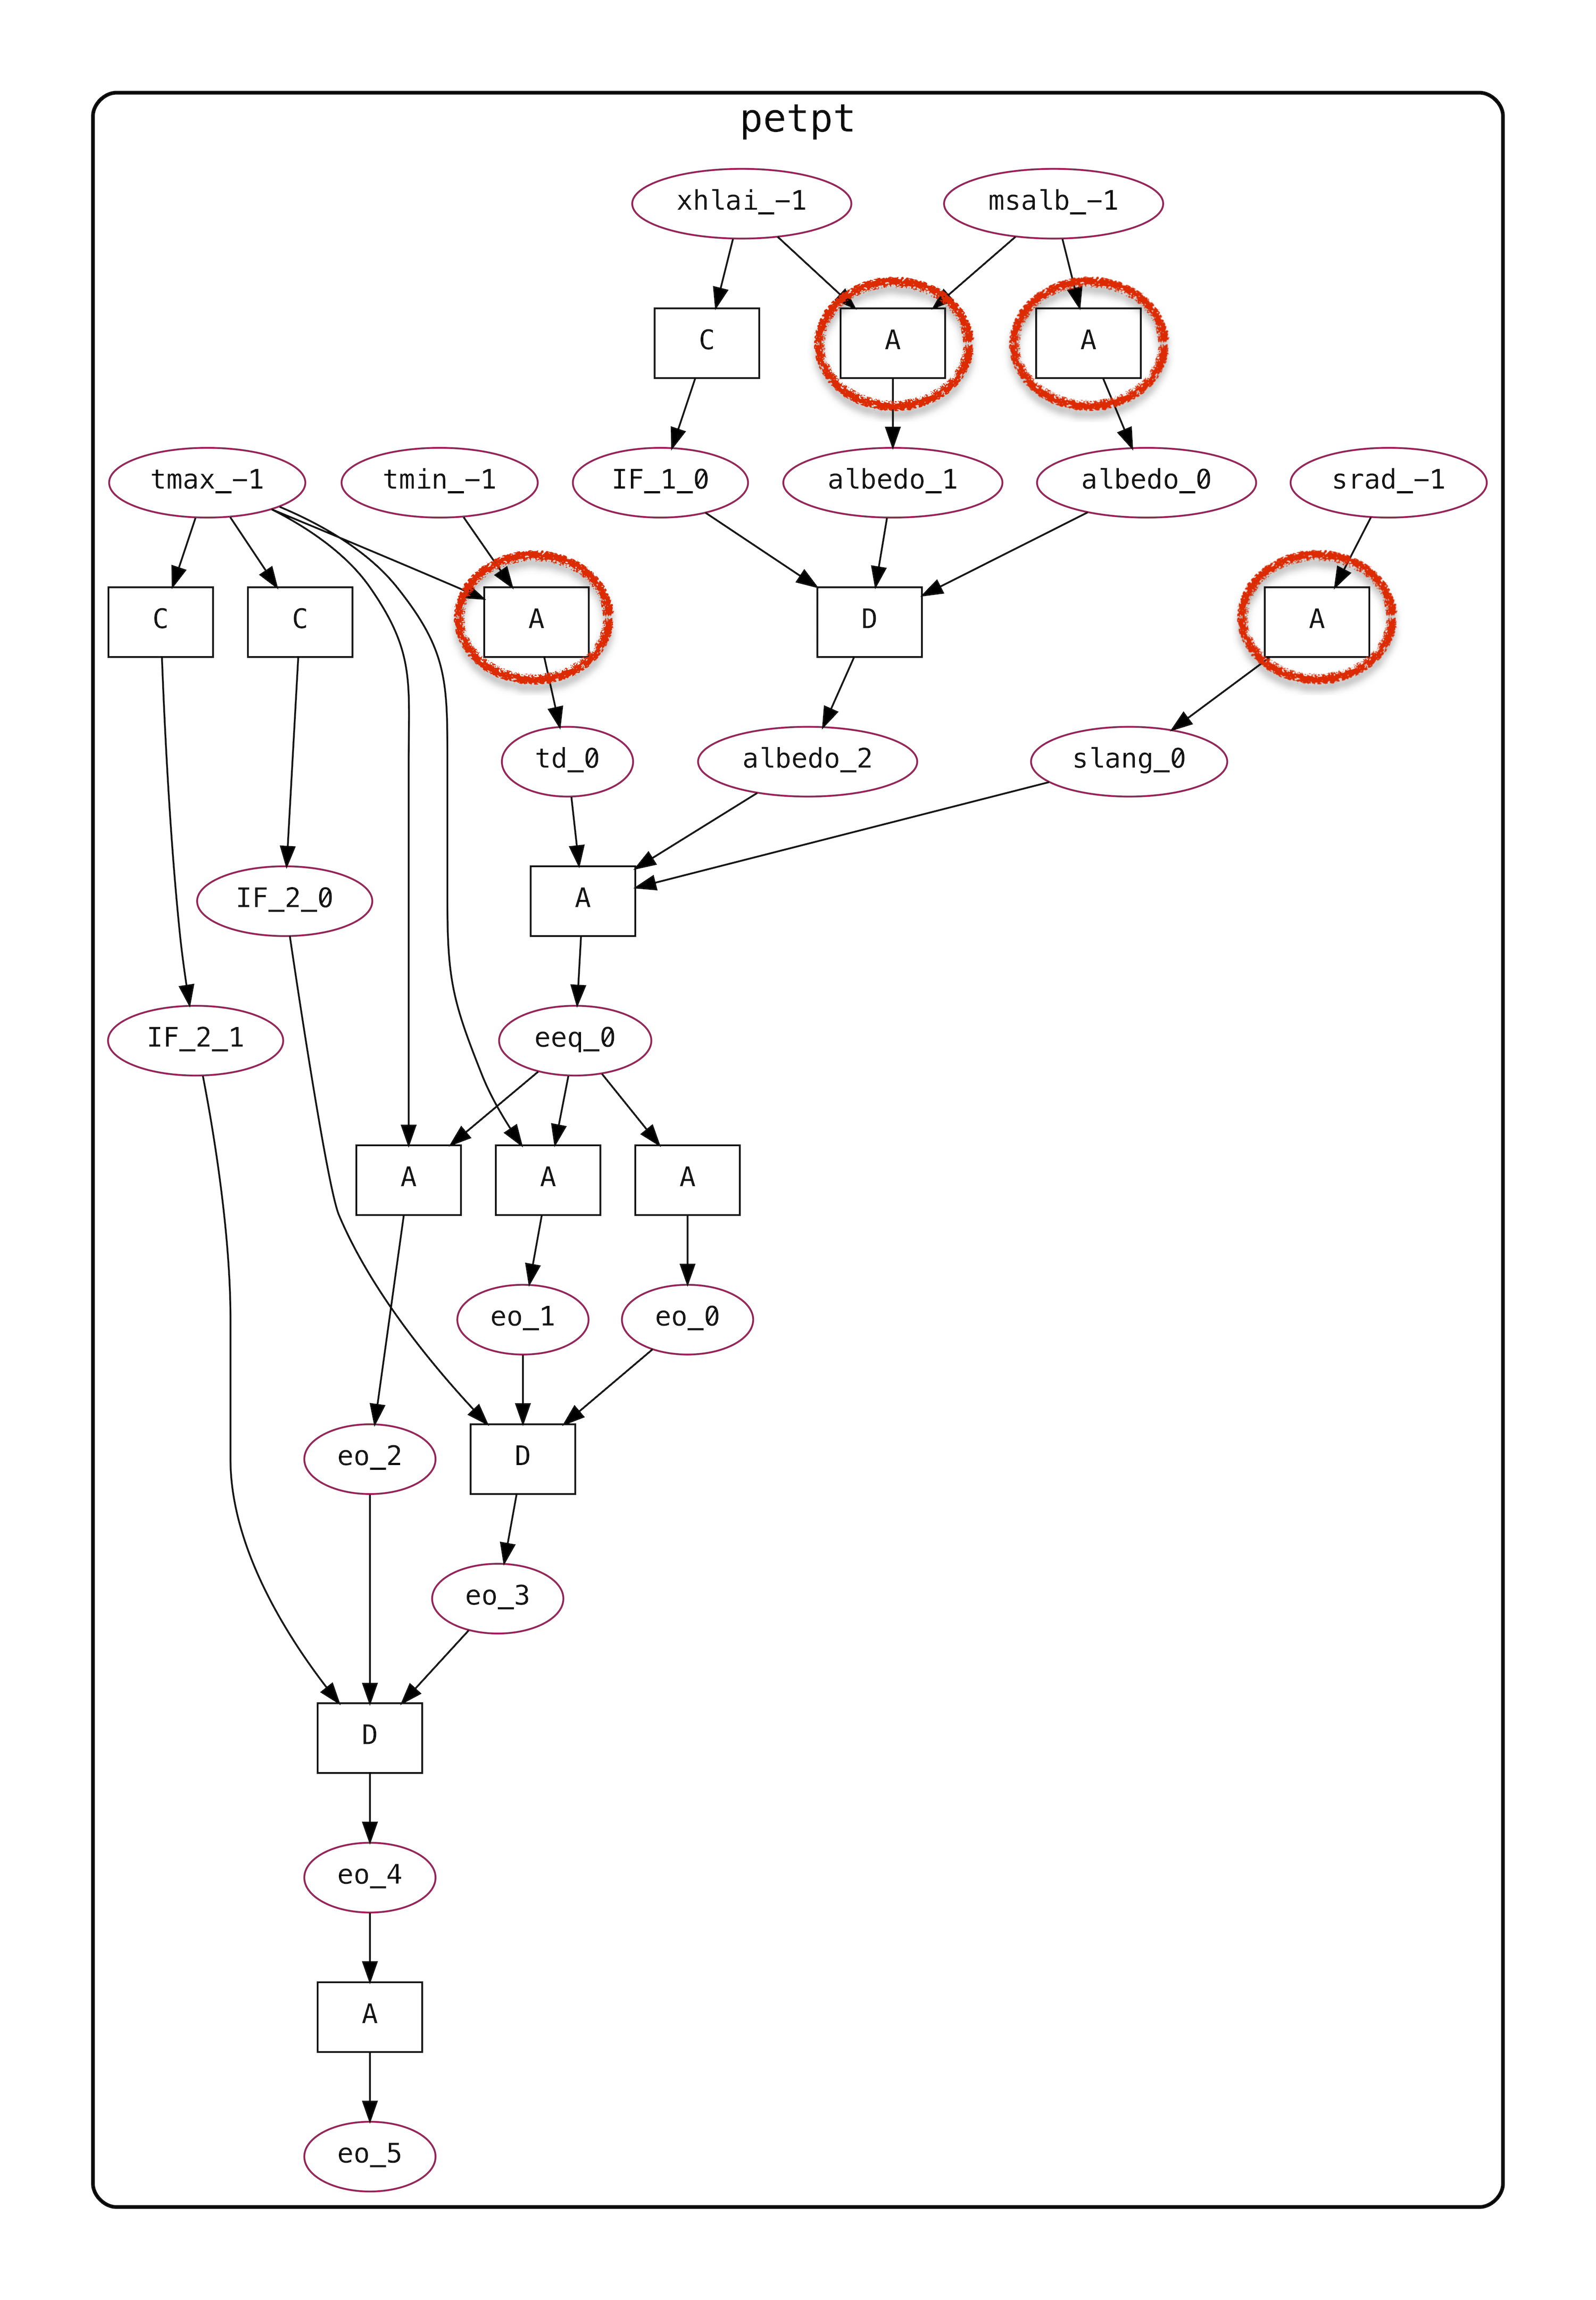
\includegraphics[width=0.45\textwidth]{PETPT_GrFN_smaller}\label{fig:petpt_grfn_cg}}
  \hfill
  \subfloat[PETASCE GrFN Computation Graph]{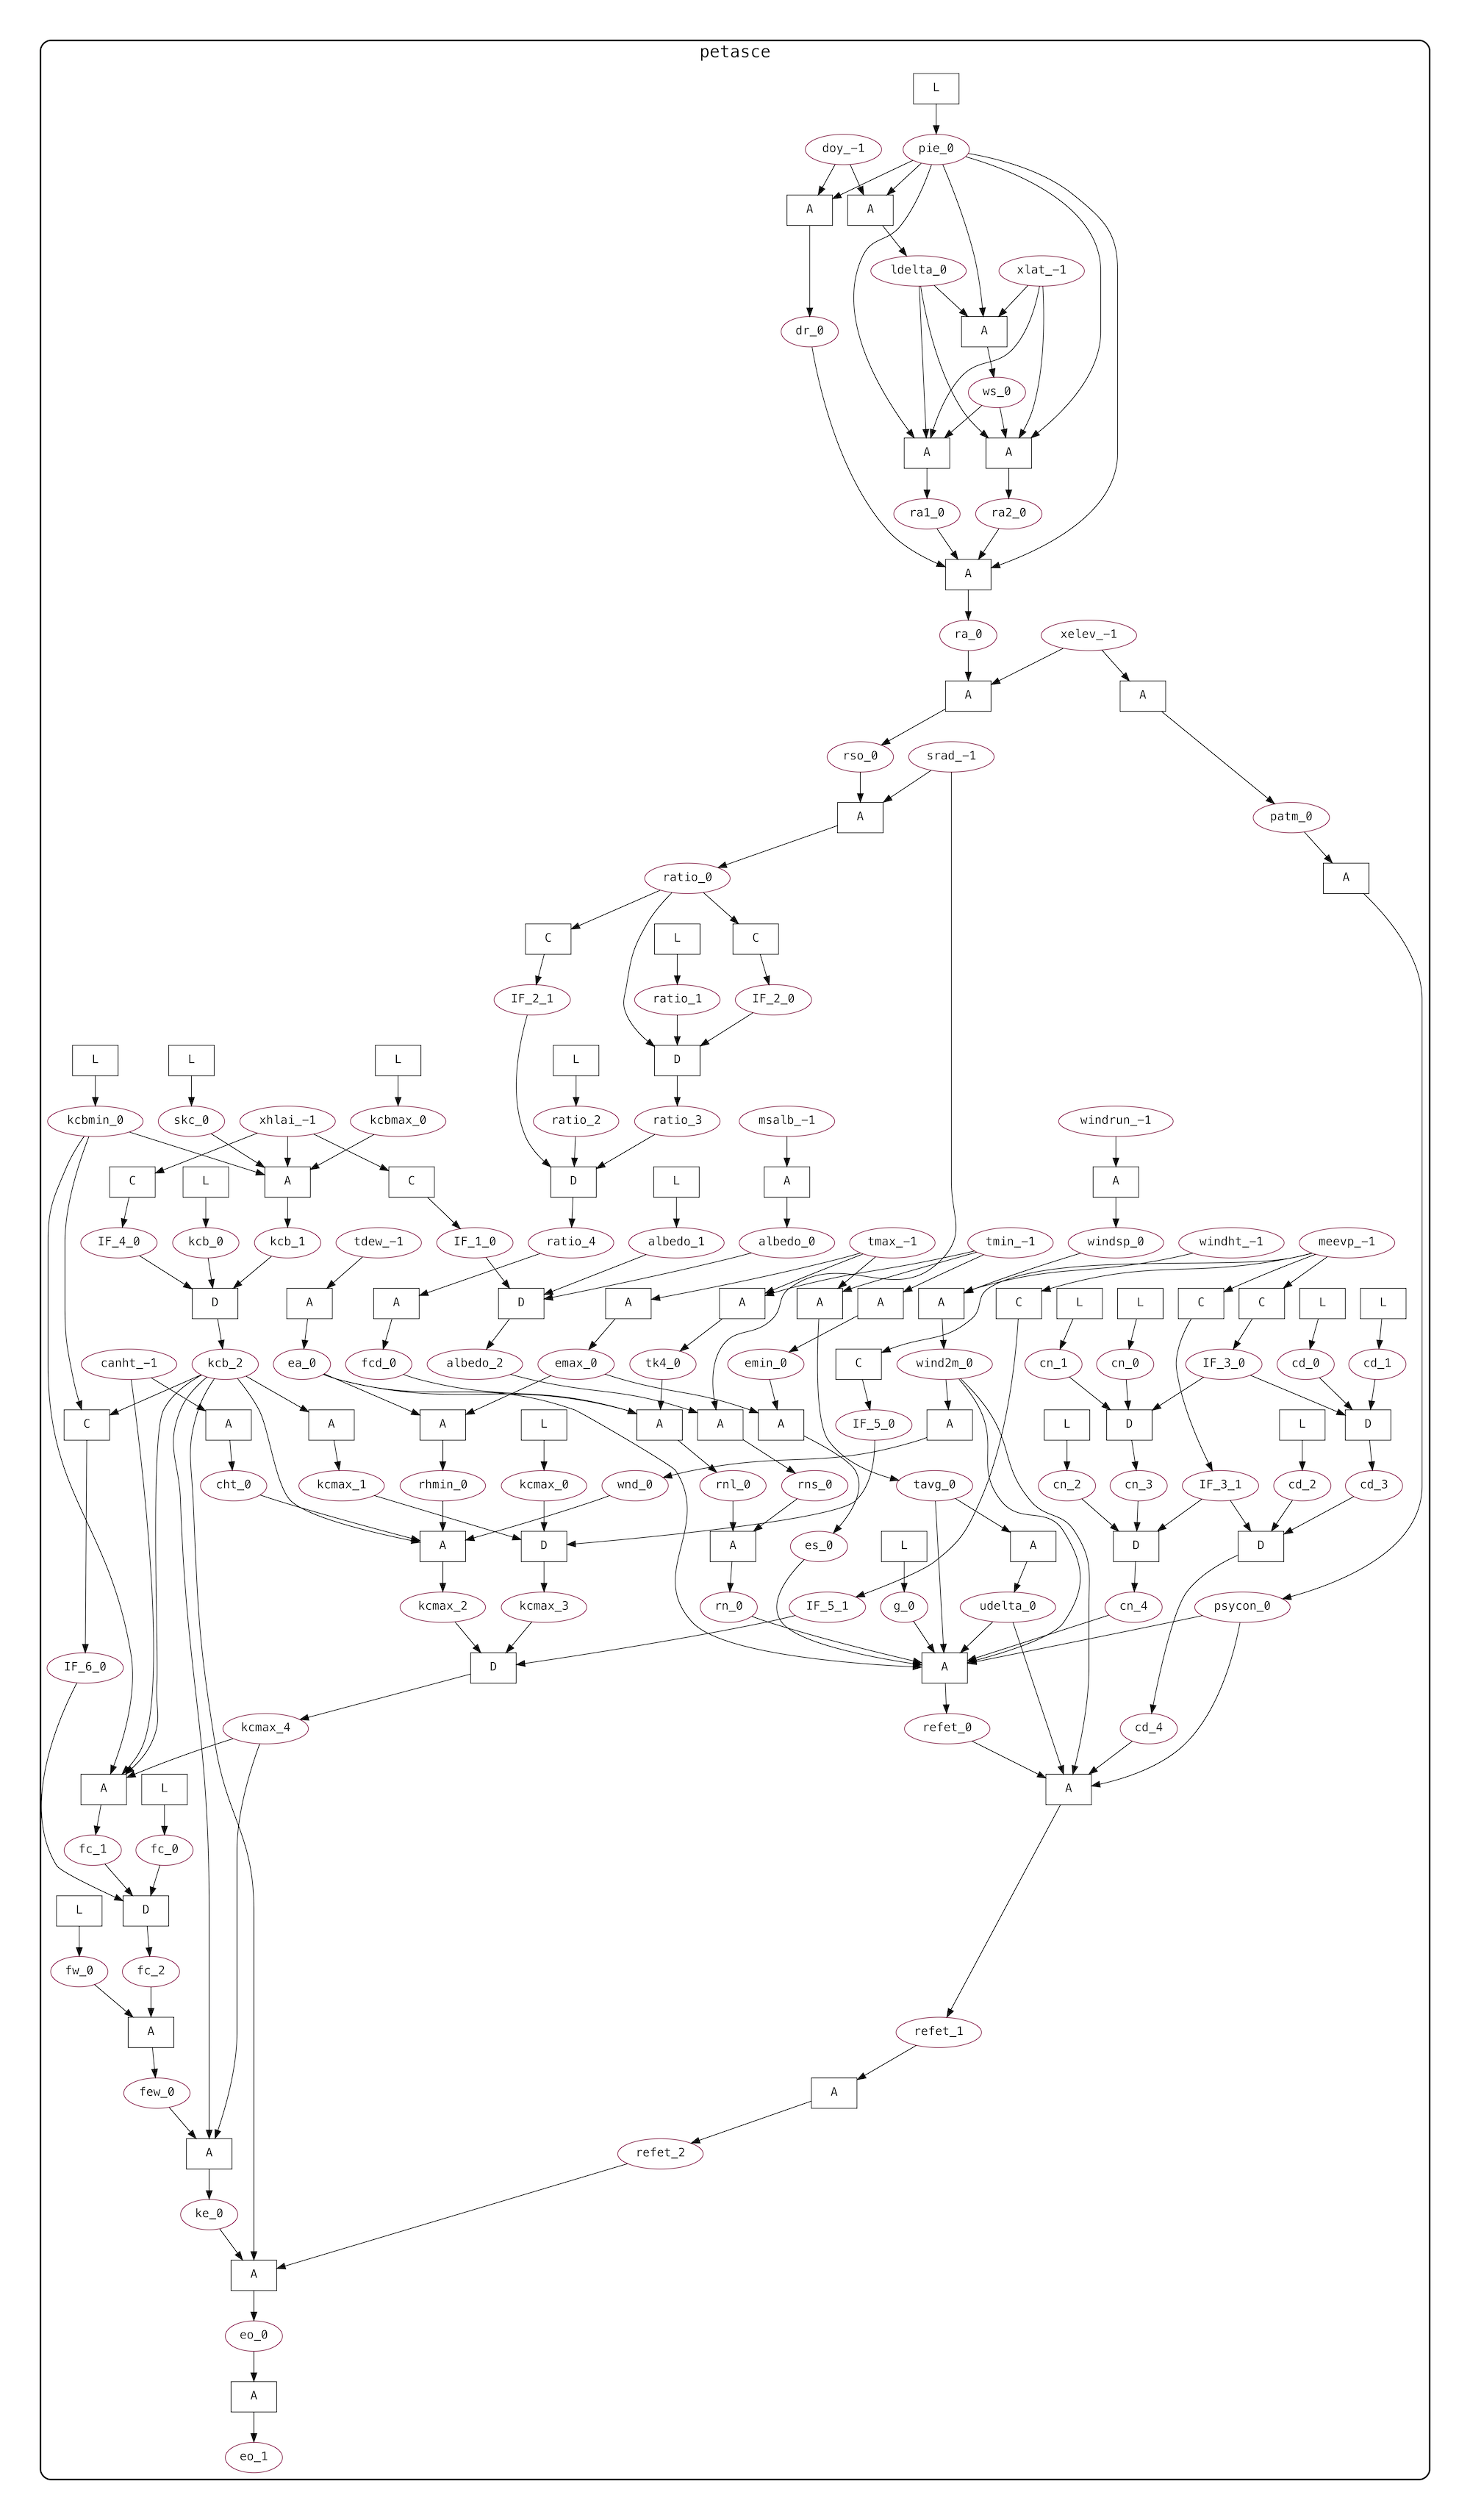
\includegraphics[width=0.45\textwidth]{PETASCE_GrFN_smaller}\label{fig:petasce_grfn_cg}}
  \caption[GrFN Computation Graph Examples]{Two examples of GrFN computation graphs \ctm{(CGs). These %The 
CG representations include the variables, represented as circle nodes, with names derived from the names extracted in the source code and variable name grounding inference; the variable names also include a numeric index representing variable state changes during processing (see text for further details).} % and include an index representing the update level of the variable found in the source code. 
Function nodes are depicted as squares with a single letter representing the type of function contained at the node. Function types include: assignment (A), conditional (C), decision (D), or literal (L). Note that in both CGs, the output nodes are variable nodes the inputs of the network can either be variable nodes or literal assignment function nodes.}
\end{figure}
\FloatBarrier

The first component of the SMS pipeline will be to develop the set of rules for how to traverse the JSON and handle the included statements to provide a clear view of how to construct a GrFN CG.
During GrFN CG construction, data-flow through the contained variables will be \ctm{represented} % handled 
by creating function nodes that contain the computations described in the lambda functions file.
In the following subsections I will present the rules for generating the control-flow structure of a GrFN CG from the associated JSON specification.

\subsection{Containers and Function Calls\label{sec:containers}}
At the top level the JSON has a list of containers. These containers represent different scope levels in the source program. A container can be a function or subroutine found in the source code or a loop. The branches of a conditional will not be considered containers due to the nature of how the GrFN will be wired to deal with conditional evaluation. a container will contain a body that will be in the form of an ordered list of statements. These statements will correspond to statements from the original source code that was present in the container. Computation graph construction will begin at a top-level container and will process through the statements in the container, constructing the computation graph as it goes. When a statement that references a new container, such as a function call, is reached the body for that statement will be processed and connected to the computation graph that is being generated. Once this task is completed, the rest of the body for the original container will be processed. This recursive process works well for traversing all containers and constructing a computation graph based upon the statements contained in each container as long as no container has a call in it's body to another container that also has a call to the original container. Unfortunately this is precisely the case with recursive functions. They act as a special case for this processing pipeline and thus they are handled separately as will be discussed in subsequent sections.

\ctm{[PAUL: Please rework this section -- I don't follow what this sentence is saying]} Landing on a function call when parsing the body of a container can be thought of as an indicator to process the body of the child container referenced by the function call.
The only intricacy here deals with the correct wiring of variable inputs into the containers plate, and the correct wiring of outputs from the container to the current position in the computation graph.
To accomplish this task a set of live variables is kept during the processing of the body of any container.
As variables are updated they carry with them an index that denotes how many updates have occurred to the variable.
Variables that are inputs to a container start with an index of $-1$ and new variables defined in a container start with an index of $0$.
Once a new container statement is reached, the collection of live variables with their current indices is past into the new container.
This permits variables to be wired appropriately across containers.

\subsection{Assignment Statements\label{sec:assg_stmts}}
\ctm{[PAUL: with a concrete example to ground this discussion, you can then point to a specific example in fortran code where an assignment is made...]}
During the processing of a container, when an assignment statement is reached it will include the following items:
\begin{itemize}
  \item A list of source variables
  \item The name of a lambda function
  \item A target variable node
\end{itemize}
Using these items the wiring for an assignment statement performs the following tasks to fully incorporate the information contained in the assignment statement into the GrFN CG:
\begin{itemize}
  \item Create a new function node for the lambda function
  \item Create a new variable node for target variable
  \item Create new variable nodes as needed for the input variables
  \item Create a directed edge from each input variable node to the function node
  \item Create a directed edge from the function node to the target variable node.
\end{itemize}
The computation required for an assignment statements can be handled by loading the assignment statement found in the source code into the function node generated during the wiring process of an assignment statement.
This allows values to propagate from the input variable nodes to the output variable node during GrFN CG execution.

\subsection{Conditional Statements\label{sec:cond_stmts}}
Conditional statements are handled via a set of two lambda evaluations.
The first evaluation is known as a \texttt{conditional} function node, that will actually evaluate the conditional property.
The second is a \texttt{decision} function node that takes as input the evaluation from the \texttt{condition} function as well as the two possible assignments for an output variable.
The \texttt{decision} function will be responsible for assigning the appropriate value to the output variable node based upon the conditional input.
Both the \texttt{decision} function node and the \texttt{conditional} function node output variable nodes as are artifacts that did not exist in the original source program.
Thus these will not be displayed when rendering the function node or variable node views of the computation graph.

\subsection{Indexed and Open-ended Loops\label{sec:loops}}
Loops naturally occur in source code as a means of expressing repetitive computations.
For the purposes of GrFN wiring, we want loops to be included, but we do not want to have backward links that would break the DAG property of a GrFN.
Therefore we will represent loops with plates that include an implicit edge back to the beginning of the loop that will be controlled by either an index or an exit condition. Therefore we will have two types of loops, the first being an indexed loop, and the second being an open-ended loop.
Indexed loops require a loop plate and have a specific index variable as well as a number of iterations through the loop.
They can easily be handled like containers as mentioned above, but require additional storage to handle information about the number of executions needed to satisfy the plate during computation.

Open ended loops will have conditional exit cases defined at a start or end point of a loop, which takes the form of an extra condition before looping or exiting the plate as compared to loops with an index and pre-defined amount of iterations.
An extra challenge is added when dealing with open-ended loops that can include multiple exit points (introduced either by \texttt{break} statements or \texttt{goto}s) as well conditional skip points where parts of the loop are skipped on an iteration (introduced either by \texttt{continue} statements or \texttt{goto}s).
This challenge will be solved by adding edges as necessary to the exit node for an open-ended loop to capture to capture the semantics of breaking and continuing.

% NOTE: section about loops from unstructured branching
In addition to explicit loops, programs can include two other forms of looping, namely \texttt{goto} statements and recursion.
In order to maximize the number of scientific models that can be expressed as GrFN the SMS pipeline will need to handle these inputs as well.
The usage of the \texttt{goto} statement has been hotly debated by computer scientists for nearly half a century.
In most modern programming languages the usage of \texttt{goto} or other such statements that allow for unstructured branching is prohibited.
However, the SMS pipeline will be used to extract models from source code inputs written in languages that do allow for unstructured branching, and thus this paradigm must be handled during the wiring phase of a GrFN computation graph.
The program analysis pipeline will handle detecting \texttt{goto}s and structuring the \texttt{goto} as an open-indexed loop.
Recursion is a commonly used software practice that must be handled for our computation graphs.
Most importantly, recursion must be identified and recursive edges that would create loops in the computation graph must be pruned.
Recursion can occur either as direct or indirect recursion.
In the case of indirect recursion a series of functions forms a loop that will repeat until a base condition is satisfied.
Identifying recursion is a task that will be handled by the program analysis pipeline.
Once a recursion loop is discovered, it will be handled the same as an open-indexed loop.
Once a \texttt{goto} or recursion loop is transformed into an open-indexed loop the SMS pipeline will handle adding it as a loop-plate to the overall computation graph in the same fashion as any other loop plate.


\section{Data Type Assignment\label{sec:data_types}}
So far I have discussed the wiring needed to create the computation graph that will allow a GrFN to be executed, and I have shown the methods necessary to make the GrFN executable. However, one more crucial component for creating a GrFN that we can perform inference upon is a discussion of how we will handle the actual data being processed from the GrFN. At the time of writing this thesis only basic data types are allowable in a GrFN. This includes numerical, string, and boolean values. These primitive data types are all singular values that represent a single phenomena, thus they match perfectly with the definition of variable nodes in the GrFN CG. The specification for each variable in a GrFN CG contains a type annotation that declares the data type of the variable. These values are derived from the JSON specification during the wiring stage of the GrFN. At execution time, these type annotations are used to validate a set of inputs and ensure proper storage format of computed variable values.

The infrastructure to represent complex data types such as Arrays, user-defined types, and unions in the AST form is still being developed by the program analysis team, and thus they will not be included in this thesis. The main challenge with representing these data types is that they are not singular variables, but are instead collections of variables. To properly perform inference over a GrFN CG all variable nodes must be singular variables, thus we cannot allow any of the above collections of variables to be represented by a variable node. This presents a problem of representation that will be studied  and resolved in future work that extends this thesis.

\section{GrFNs are Dynamic Bayes Nets\label{sec:grfn_as_dbn}}
Once we have extracted a GrFN CG that represents a scientific model we will want to analyze the model and compare it to other existing models.
Both of these tasks require us to be able to perform inference on the GrFN CG by observing the behavior of the model over a distribution of inputs.
A well defined methodology for performing inference over DAGs is to establish the DAG as a bayesian network \citep{bishop2006pattern}, a type of probabilistic graphical model, and then to use the robust set of methods associated with bayes nets to solve inference problems.
In this section I will now demonstrate how a GrFN CG is a bayesian network in order to unlock the use of inference on GrFN CGs.

A GrFN CG has a set of input variables that are wired as a network to the outputs of the model represented by the GrFN CG.
The inputs of the GrFN CG can be assigned values and will then return an output value for each of the GrFN CG outputs.
Recall that all variables in a GrFN CG are treated as random variables.
Bayes nets have a set of variables that are linked to observable random variables that exist in the real world.
This presents a challenge for representing a GrFN CG as a bayes net because several variables in a GrFN CG represent the same natural phenomena.
However, we can view a GrFN CG as a \ctm{\emph{Causal Analysis Graph}} (CAG) that allows us to visualize only the variable relationships present in the GrFN.
Below are the CAG views for the two GrFN CGs under study in this thesis. Notice that inspecting this view gives us a graph structure that looks similar to a bayes network that has loops (i.e. one that can be unrolled over time).

\FloatBarrier
\begin{figure}[!tbp]
  \centering
  \subfloat[PETPT GrFN CAG]{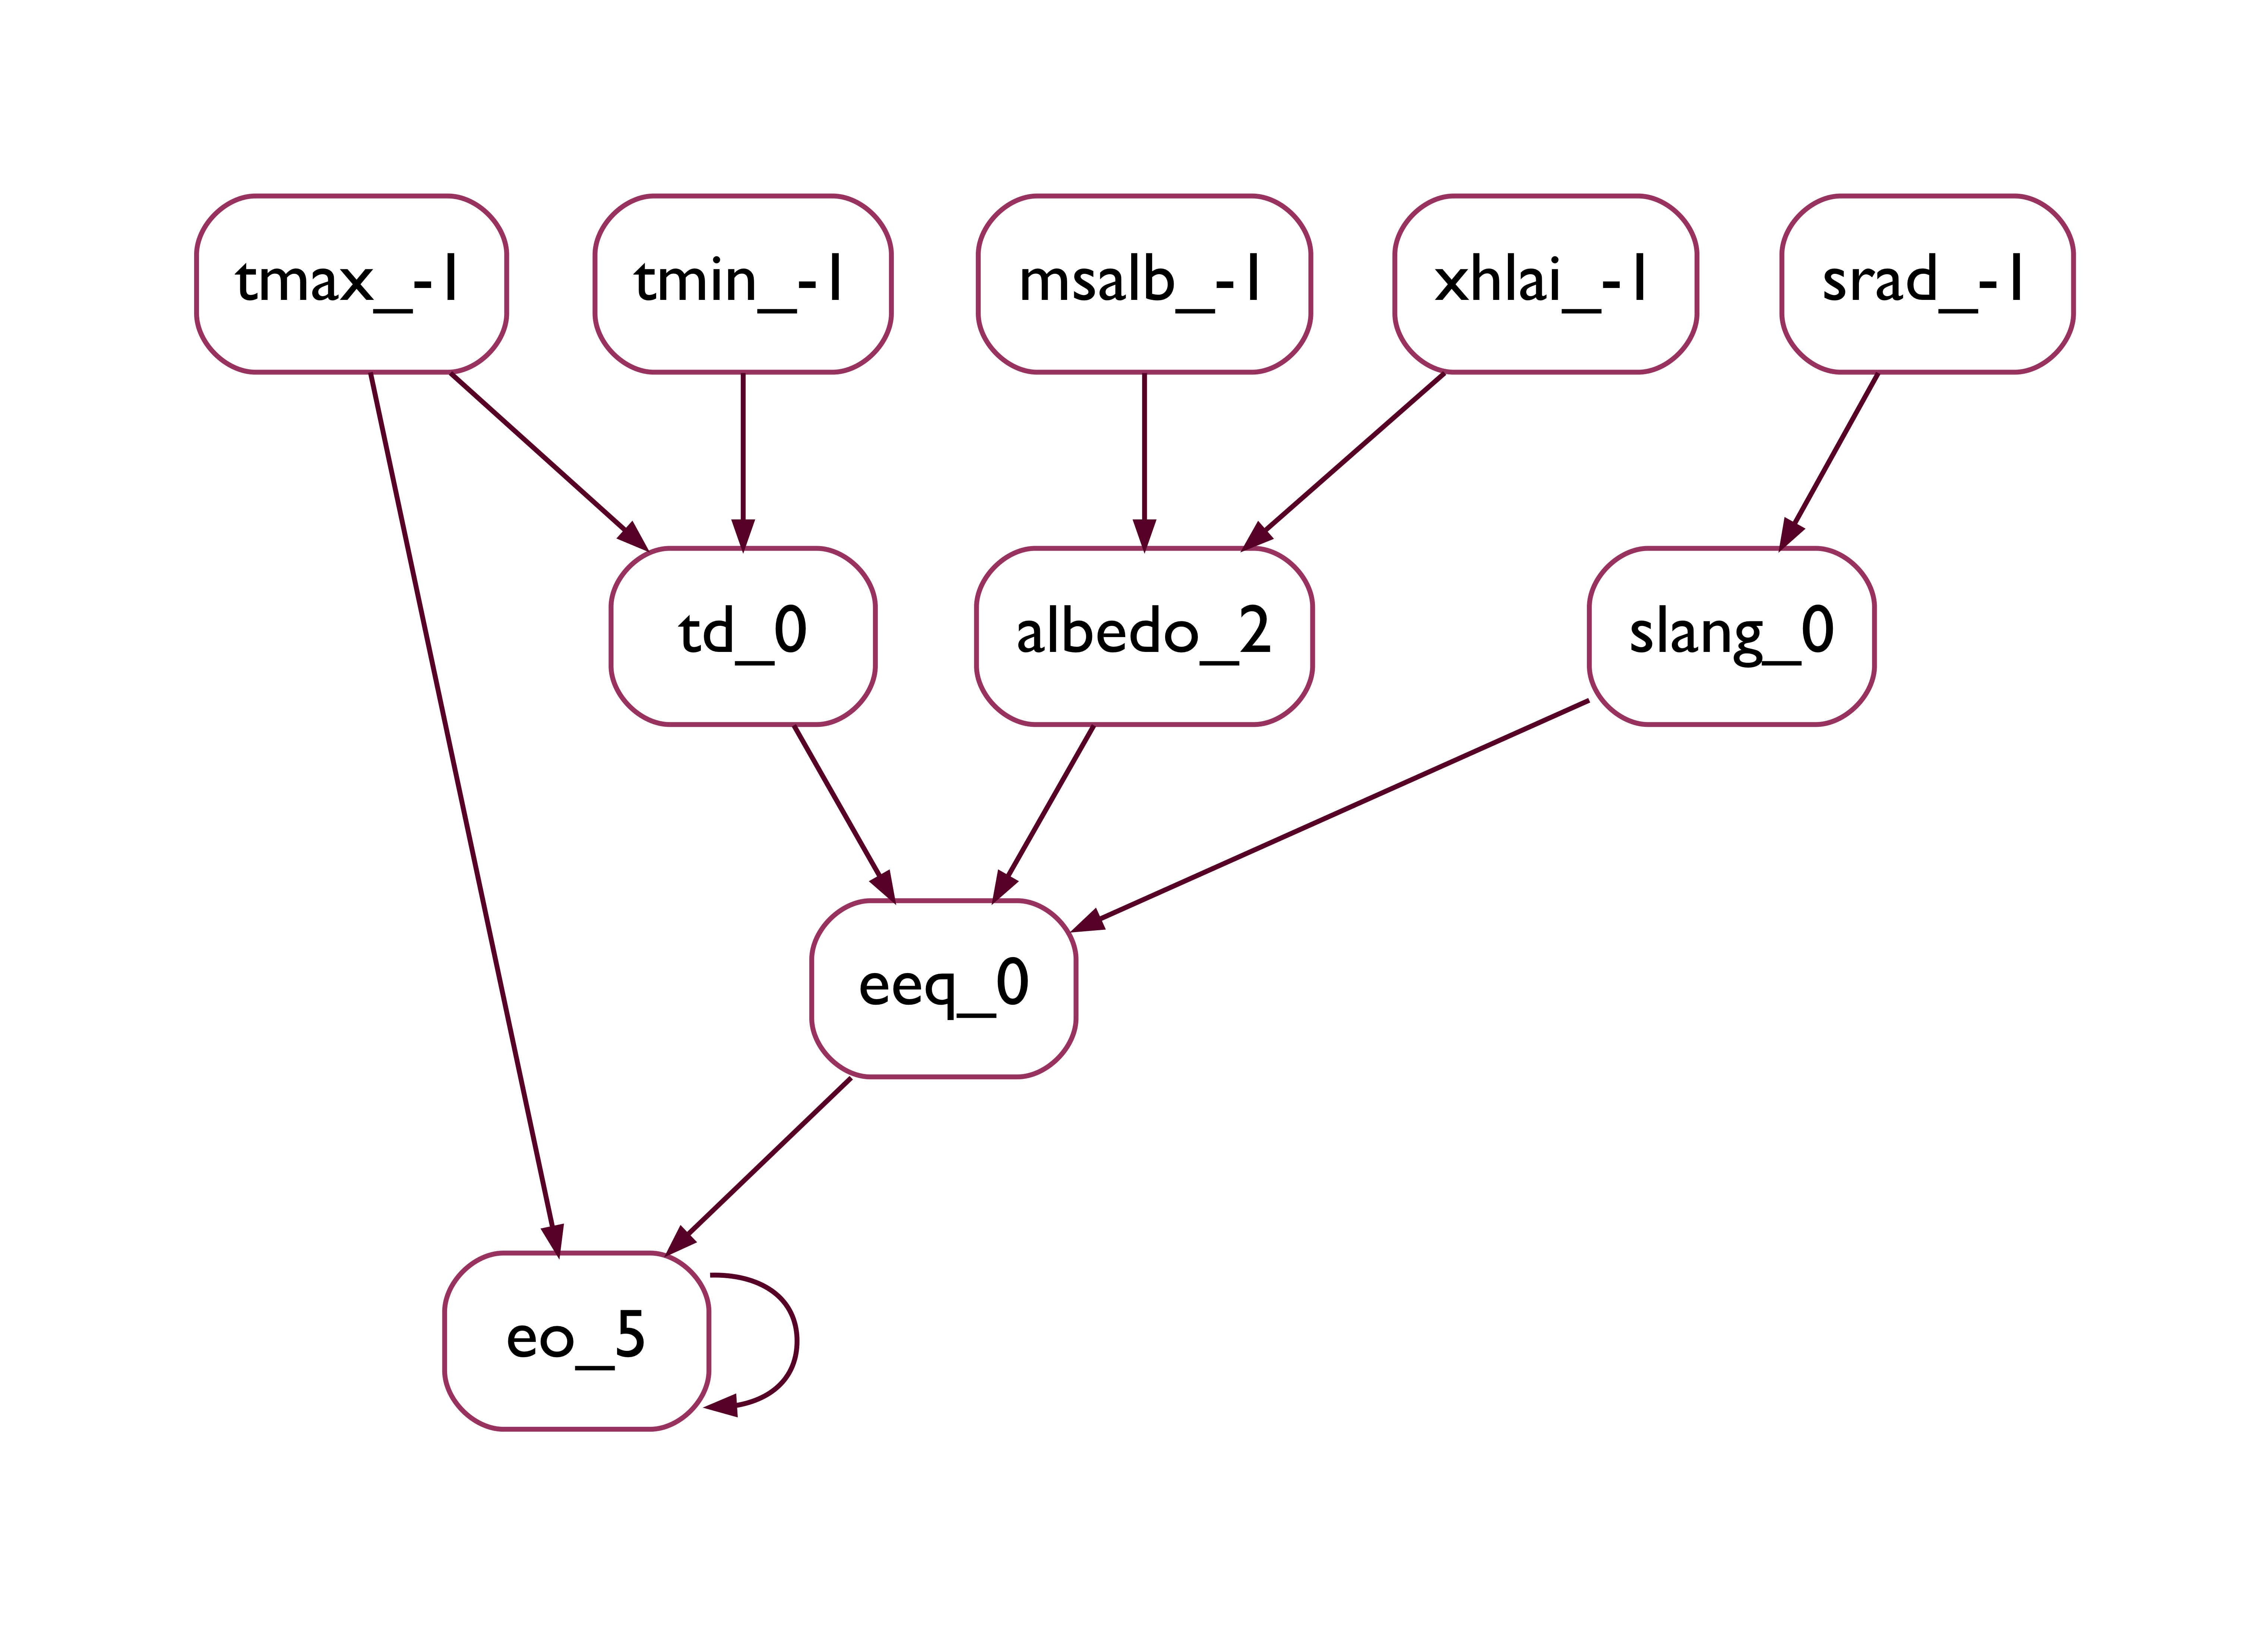
\includegraphics[width=0.75\textwidth]{PETPT_GrFN_CAG}\label{fig:petpt_cag}}

  \subfloat[PETASCE GrFN CAG]{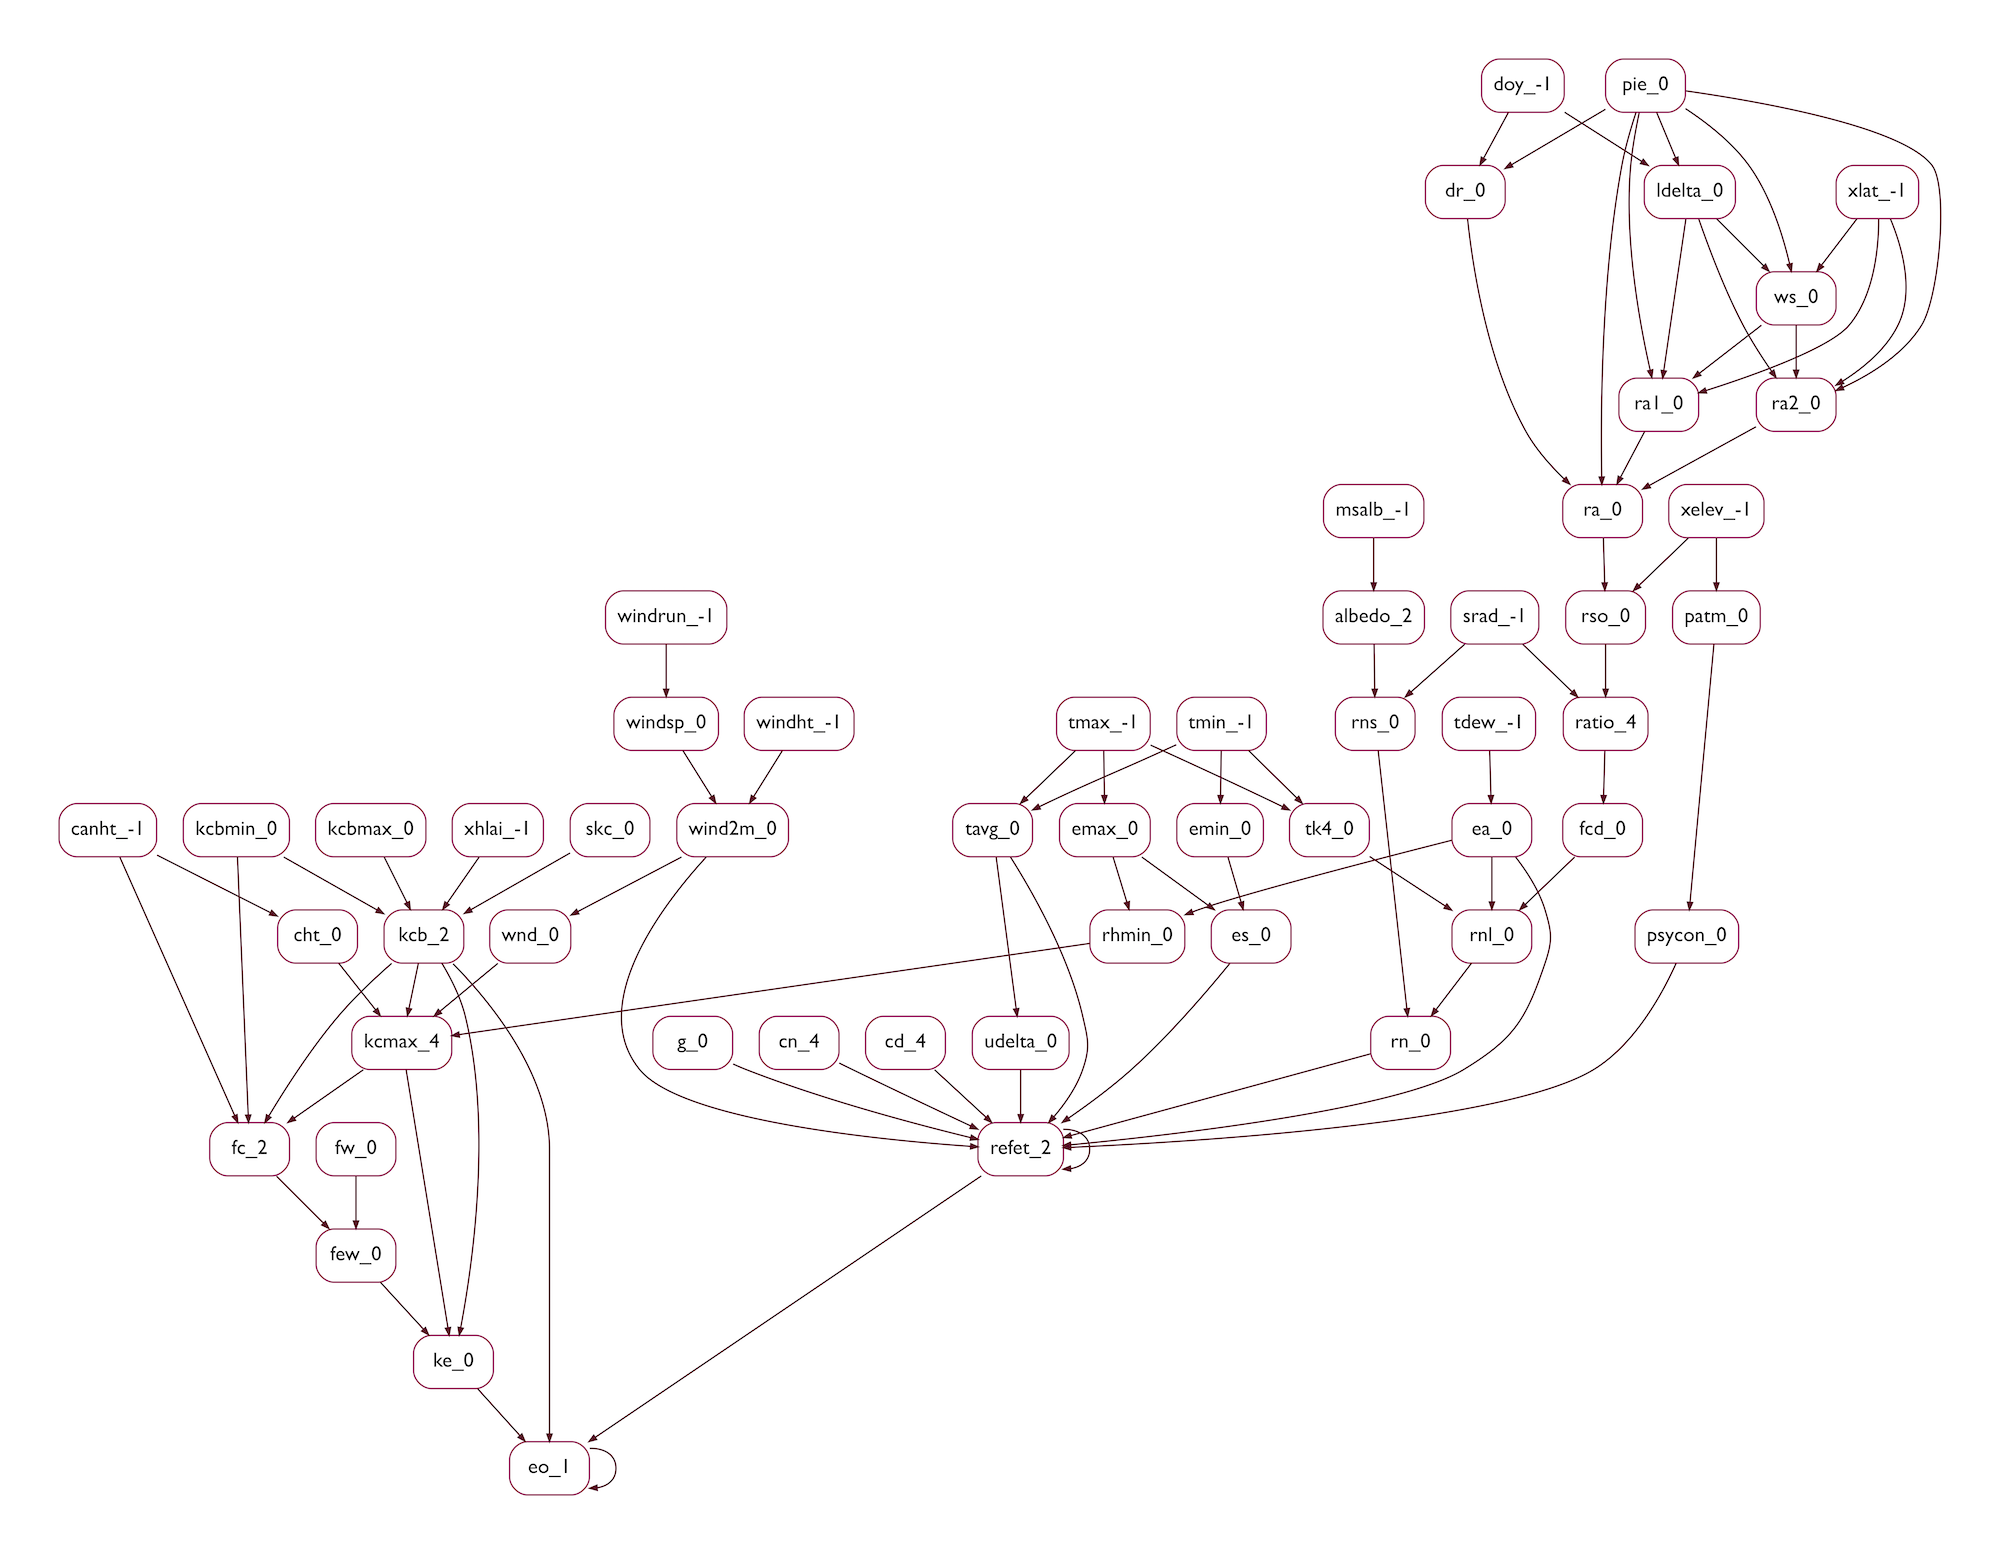
\includegraphics[width=0.75\textwidth]{PETASCE_GrFN_CAG_smaller}\label{fig:petasce_cag}}
  \caption[GrFN Causal Analysis Graph Examples]{Causal analysis graph views of the PETPT and PETASCE evapo-transpiration models.}
\end{figure}
\FloatBarrier

When treating the input variables as random variables we can induce a distribution over the values that they can take.
This distribution will then permeate through the function nodes to the other variable nodes in the GrFN CG.
For the GrFN CG to be a Dynamic Bayes Net (DBN) we need the probability distribution of the output variable to be a product of all of the input probability distributions \citep{pearl2009causality}.
During the computation of any inner variable in a GrFN CG we have a lambda function that denotes how the the inputs to the computation are to be combined to form the output.
All possible combinations are mathematical functions, that are able to be applied over the probability distribution of the inputs.
Therefore the resulting computed inner variable has a distribution that is the combination of the distributions over the inputs.
However, this distribution is not yet a probability distribution.
In order to create a probability distribution a normalization step is required so that the total probability mass sums to 1.
Once this step is complete we can see that we have satisfied the requirements for a DBN for the trivial case of a single computed node with a set of input nodes.
Since we are free to induce distributions on the input nodes of a GrFN, and all inner nodes and output nodes of a GrFN are defined in the same manner as the case explored above we can conclude that a GrFN CG is indeed a DBN.

\section{GrFN Computation Graph Execution\label{sec:cg_execution}}
Once the wiring stage for a GrFN has been completed, the GrFN CG must be made executable. The execution of a GrFN CG requires the execution of all functions stored at the function nodes of the computation graph. Therefore the problem of executing a GrFN CG can be simplified to the problem of determining an ordering of execution of the function nodes that allows for all of the function nodes to be executed without any failures. Of course a GrFN CG also needs to save the state of variables during execution in a way that allows the function nodes to access the information stored for each variable they require. In this section I will present the methods developed for the GrFN CG to handle the function evaluation ordering problem and the variable storage access problem.

\subsection{Call Stack Creation\label{sec:call_stack}}
Creating a computation graph from a GrFN specification allows us to formally represent an extracted scientific model as a graph data structure.
However, if we wish to analyze the extracted model, then we will need the ability to compute information over this data structure.
To accomplish this we introduce the idea of execution over a computation graph. The computation graph contains a set of function nodes.
Computing the lambda function stored at each function node is analogous to executing the computation graph from the set of inputs to the output.
However, the function nodes rely upon having values populated at each of their input variable nodes in order to perform their computation.
Therefore the task of executing a GrFN CG can be rephrased as determining how to order and execute the functions nodes contained in the computation graph.

A Naïve first-pass solution to accomplish this goal would be to use a graph traversal from the output to the inputs where at each function node, the node will determine whether values for each input variable node have been populated.
For any input variable nodes that have not been populated, the function node will call the parent function node responsible for computing the value of the input variable node.
Once all such calls have returned, the function itself will evaluate. This recursive calling procedure is very similar to message-passing, a method for inference on factor graphs.
While this will ensure correct model execution, this method of handling execution is not as efficient as possible.
To start the recursive call structure adds additional function setup and calls to the execution, on the order of the number of functions included in the computation graph.
The second obvious inefficiency with this execution is that the recursive operations must be done for each execution, and they require all function nodes to be executed sequentially.

These two concerns can be addressed by creating a call stack comprised of all the function nodes contained in the GrFN CG.
The order of computation between function nodes implies that the call stack is equivalent to a partially ordered set (poset) upon the function nodes \citep{simovici2008miningTools}.
Once this poset is recovered, execution of the GrFN CG can occur by executing all functions at the first level in the poset, then moving to the next level in the poset, and then repeating the sequence until reaching the end of the call stack.
This allows all function nodes at the same level in the poset to be executed concurrently, and the computation required to create this call stack only needs to occur once.

Computing the call stack requires a series of separate computations.
First a control flow graph (CFG) \citep{allen1970CFG} must be extracted from the GrFN CG.
As defined above, the GrFN CG is bipartite with respect to the variable and function nodes, such that no variable node is adjacent to another variable node and vice-versa for a function node \citep{bondy1976graph}.
Therefore a GrFN CFG can be extracted from the GrFN CG by simply squashing any variable node between a pair of function nodes into a singular edge connecting the two function nodes.
Since the GrFN CFG is derived from the GrFN CG it will have a set of input nodes.
Starting from this set of input nodes an index is assigned to each node, beginning at zero.
Each time an edge is traversed the index increases.
If a function node is reached and it already has an index the index is updated to the maximum of the current index and the newly calculated index.
Once the full graph traversal is complete we have an index for the poset.
Function node sets are created according to the index values, and the index values also provide the ordering of the function node sets.
Smaller index values correspond to the function node sets that are to be computed first.
Function sets can then be placed into the call stack by pushing the sets with the largest index value onto the stack first.
The GrFN CG now has access to a call stack that can be used to execute an input set.
During execution, when the call stack is being used, it can be maintained by pushing popped values from the stack onto a different empty stack.
After execution, the values can be popped from the temporary stack and pushed back on to the original call stack. This ensures that the call stack order will be maintained for the next execution.

\subsection{Computation Graph Input Execution\label{sec:input_execution}}
During execution, a GrFN utilizes a value storage tag at each variable node.
During computation, function nodes pull their input data from the value tag of each parent variable node of the function node.
The output from the function node is stored in the value tag of the variable node that is the child of the function node.
Function nodes are guaranteed to have access to the variable node input data at the time of their execution by the call stack execution order discussed in the previous section.
After all function nodes have been executed the output variable node of the GrFN CG will have the computed output value stored in its value tag.

While a GrFN CG is perfectly capable of executing one set of inputs at a time, as described in the method above, the CG can also handle executing over multiple sets of inputs at once.
The SMS pipeline accomplishes this by making use of the PyTorch tensor computation framework.
It is advantageous to compute multiple inputs at once using vectorized computations because pooling like computations lowers overall compute time.

\section{Model Overlap Identification\label{sec:overlap_identification}}

While analytical methods can provide a large amount of useful information to modelers about a single model, the real benefit of the AutoMATES system comes from the ability to automate comparisons among competing models. Competing models can be identified from the output variables of their computation graphs. After identifying a selection of competing models the comparison phase can begin.

For any two competing models of the same phenomena the comparison phase consists of the following:

\begin{enumerate}
  \item Identify the overlap between the variables in each models computation graphs. This corresponds to overlap in observable real-world phenomena.
  \item Extract the sub computation graphs for each model based on the variable node overlap.
  \item Perform analysis on the overlapping computation graphs and compare the results with the analysis results from the models whole computation graphs.
\end{enumerate}

In order to accomplish the tasks outlined above, I will introduce a new construct, known as a Forward Influence Blanket (FIB). A FIB is a specific instance of a Markov blanket \citep{pearl2009causality}, derived from a GrFN computation graph, that can be used for forward analysis.  % TODO: possibly define forward analysis and markov blanket
After the completion of these tasks the information gained from the comparative study of these models can be added to the final model report, or used for automatic model selection. In this chapter I discuss model comparison in terms of two models compared directly with one another. At the end of the chapter I will elucidate on the necessary steps to generalize this form of binary model comparison to a set of $N$ models.

\subsection{Identifying a Forward Influence Blanket\label{sec:fib_creation}}
Imagine the structure of two computational models of the same phenomena in the most general sense. We can say with certainty that both models will have the same output variable, namely the variable that represents the phenomena of interest. From this there are three options for how the set of input variables between the two computational graphs can overlap. The least interesting option is that the two models could share no inputs variables. This would mean that the computations involved in each model are wholly independent and could be combined if necessary in a trivial manner, at least at the input level. The more interesting option is that a subset of the inputs are shared between the two models. This entails that the models will make use of the same data, though the computations used to transform that data into a model output will almost certainly differ. It is possible that the set of input variables will overlap exactly between the two models; however, it is much more likely that there will be some input variables that are not contained in both. In the following subsections I will discuss how to build a computation graph that represents the computation present in a GrFN that corresponds to utilization of shared variable nodes with another model.

% TODO: Add material about Shared Structure Identification here
The shared structure components of a FIB for two models of the same phenomena are identified using the following strategy.
By definition the models share the same output variable node.
Therefore any shared structure will be within the range of a shared variable node, either an input variable or an inner variable node, and all the full computation path to the output node.
A set of shared nodes between the two graphs can be discovered using node name matching on the grounded node names.
This is done upon the CAG view of the GrFN CG so that variable nodes are only matched once and not once per update recorded in the overall CG.
Using the set of shared nodes and the output node we can discover all computation paths that lead to the output node by doing an exhaustive path search from each shared node to the output node \citep{sedgewick2002algorithmsInC}.
Combining the outputs from all of these paths together gives us the shared portions of each GrFN CG that serve as the basis for each models FIB.

% TODO: The section discusses Cover Set Variables
The key aspect of a FIB that distinguishes it from a GrFN computation graph is that the portions of the original computation graph that are not shared between the two models under comparison are pruned.
In order to ensure that the resulting models are still executable, variable nodes representing new inputs to the FIB computation graph must be retained.
This set of variables has been identified as the cover set.
Forming this cover set and adding it to the shared overlap portion of each GrFN CG as mentioned above is the last step necessary to fully create the FIB for each model.
Identifying a variable as being a member of the cover set stems from the initial shared graph structure extracted from the original GrFN CGs.
All nodes along the shared structure must be compared to the node structure in the original CG.
If any nodes are missing a branch that is present in the original CG then the immediate parent of the node must be added to the set of cover nodes and is grafted on to the FIB.
Once the set of cover nodes are added to the shared graph structure the FIBs for each model are complete.
To visualize what a FIB looks like for both a small and large CG we have added the FIBs that denote the overlap between the two evapo-transpiration models.

\FloatBarrier
\begin{figure}[!tbp]
  \centering
  \subfloat[PETPT FIB CAG]{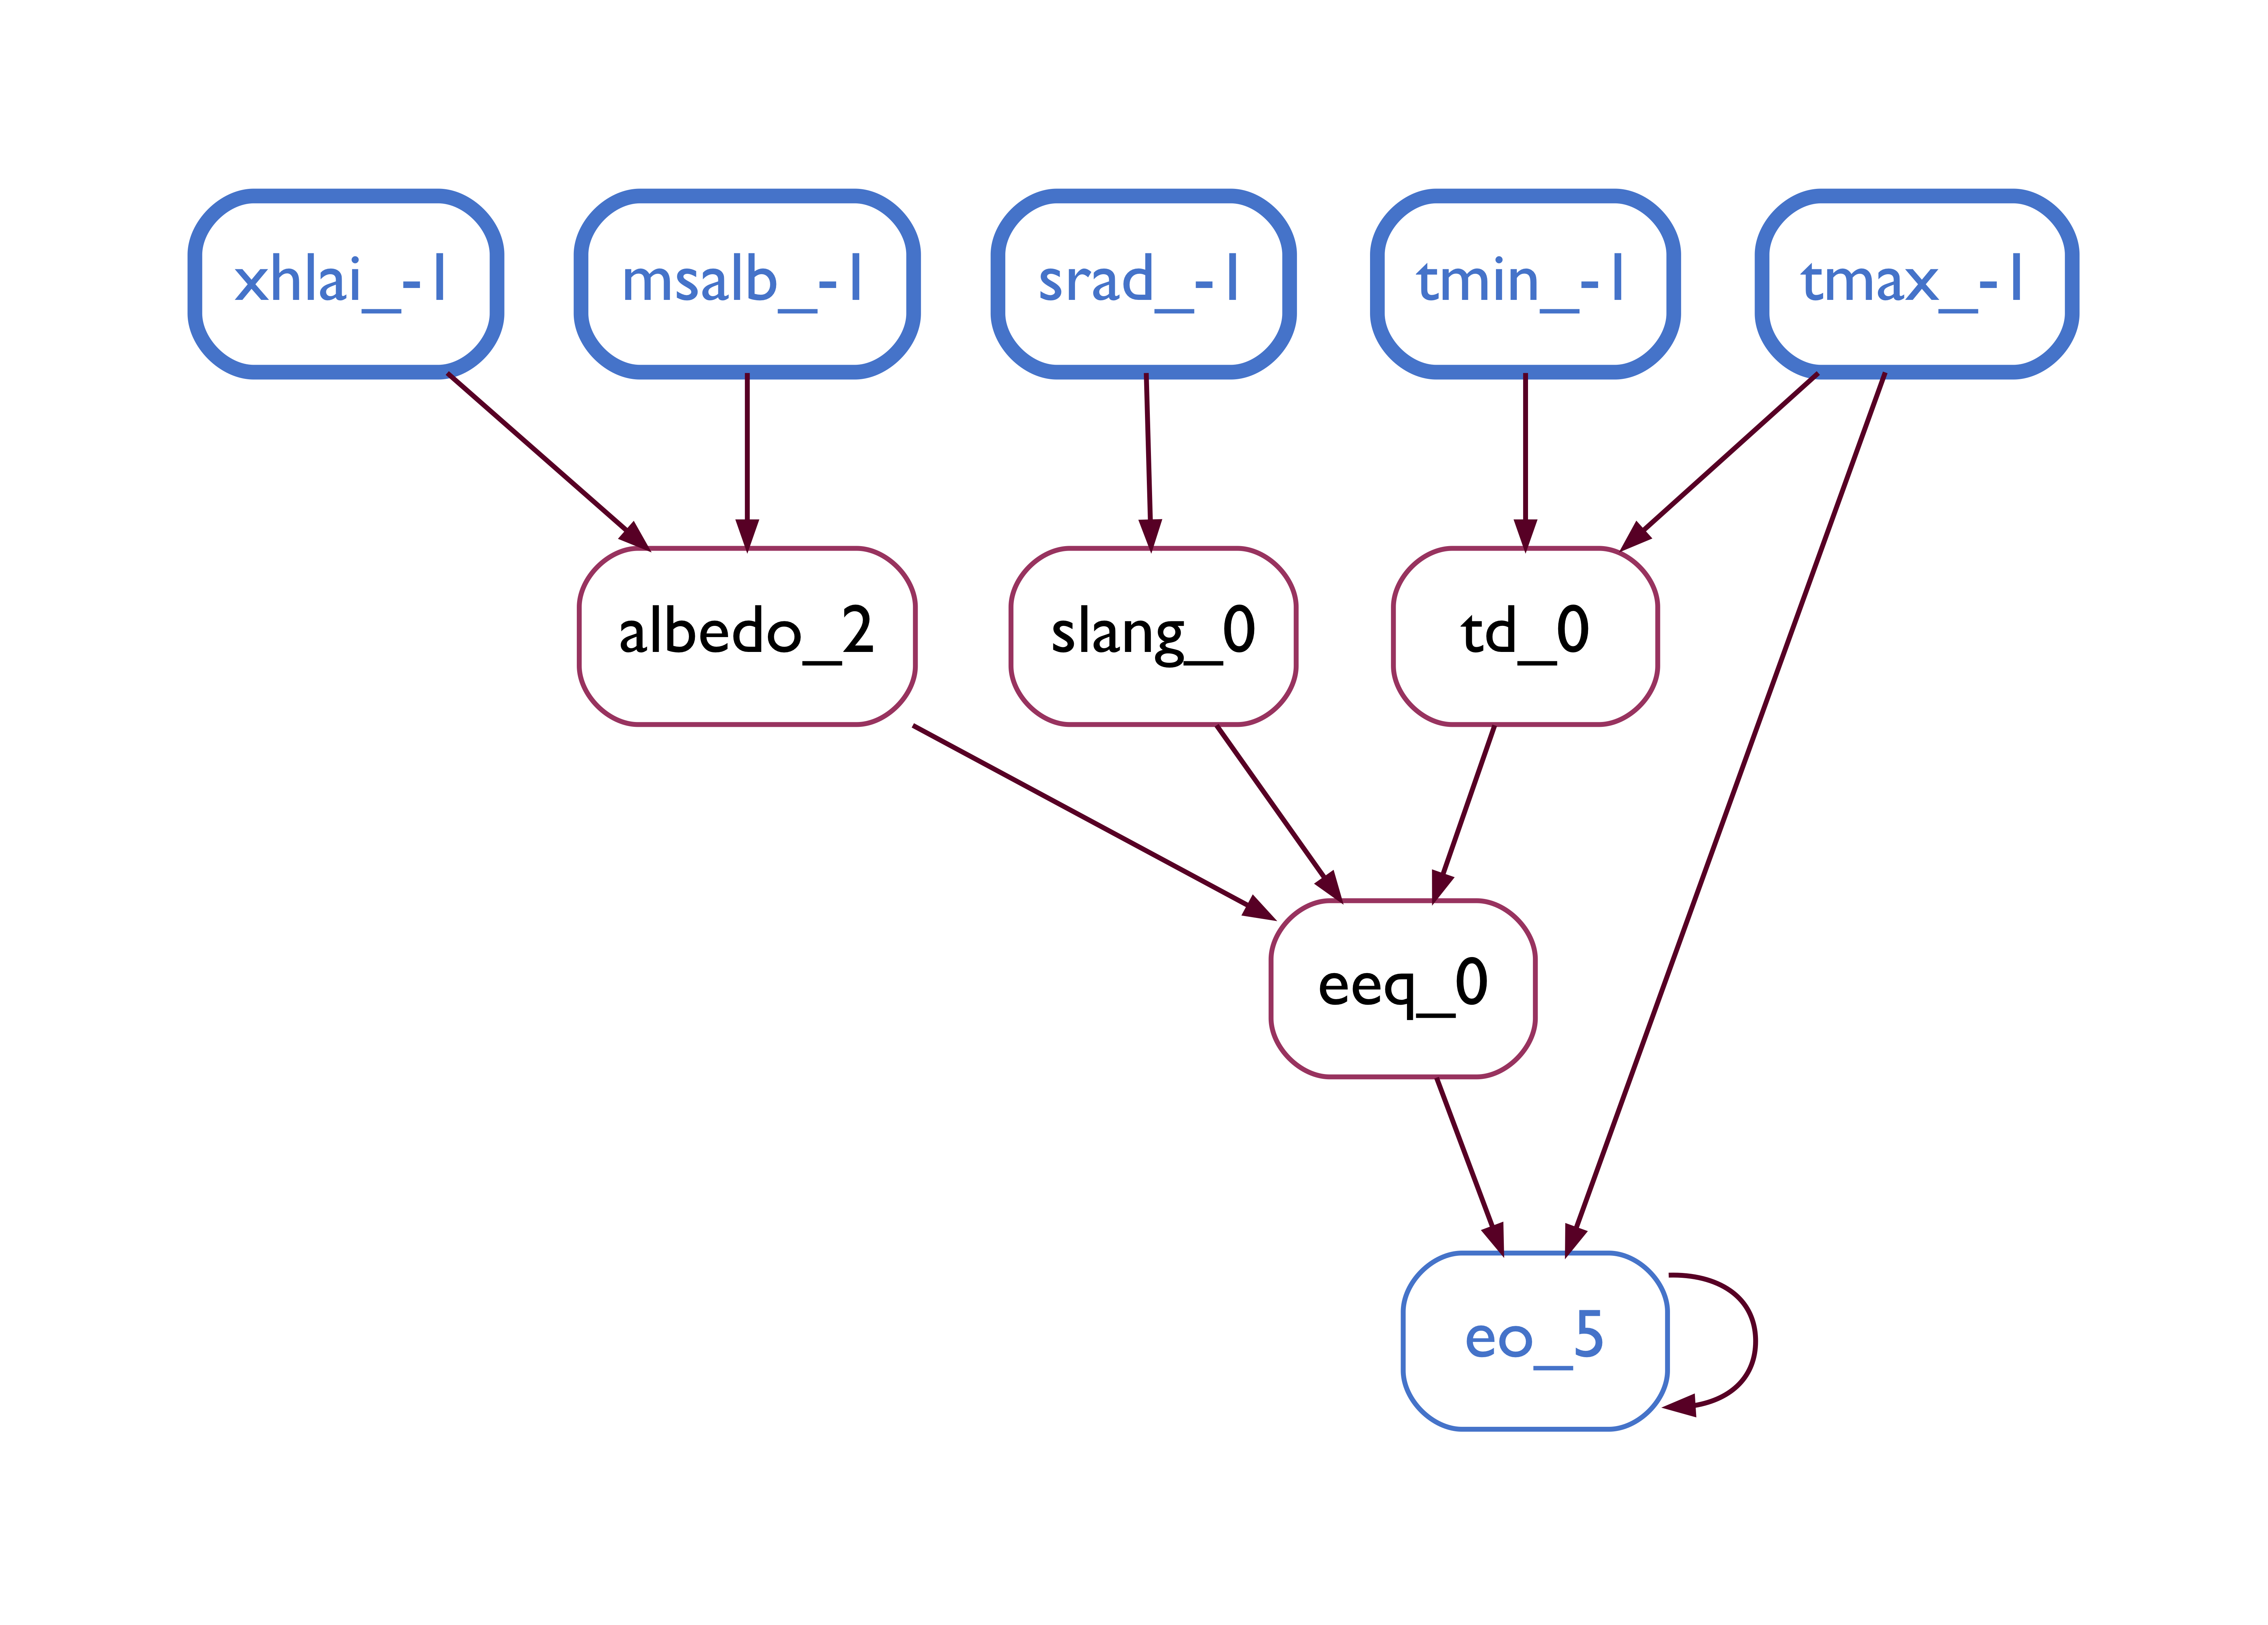
\includegraphics[width=0.75\textwidth]{PETPT_FIB_CAG}\label{fig:petpt_fib}}

  \subfloat[PETASCE FIB CAG]{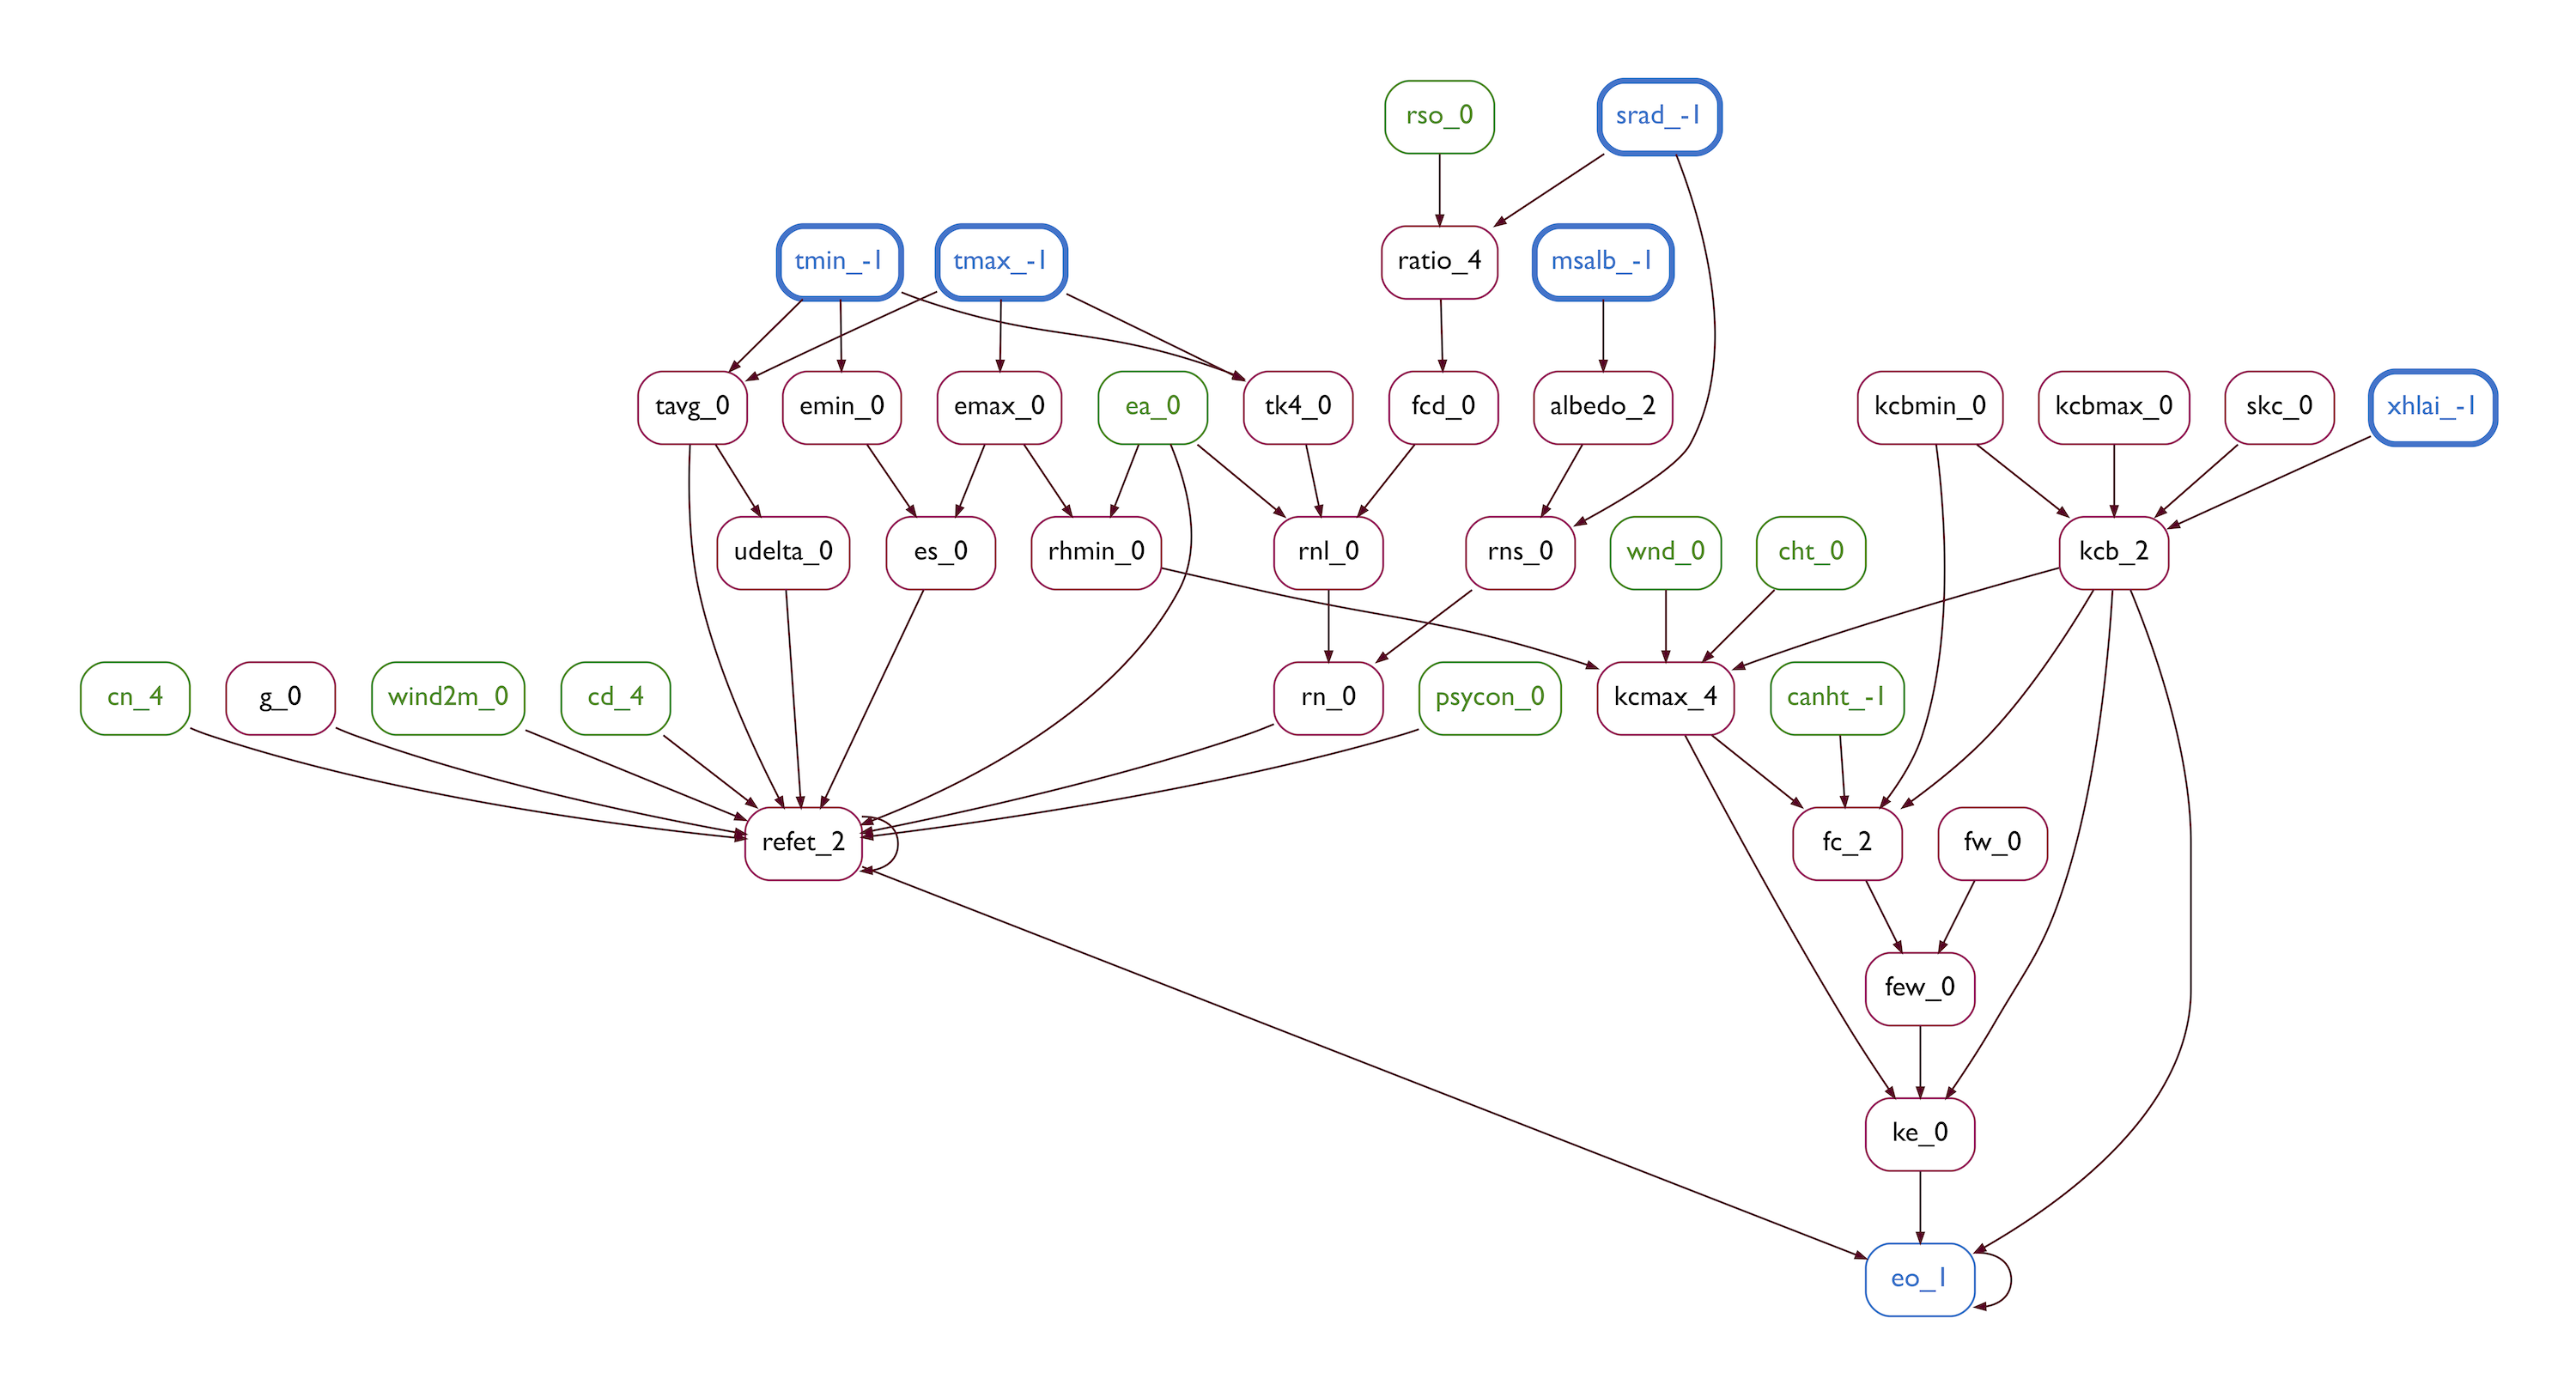
\includegraphics[width=0.75\textwidth]{PETASCE_FIB_CAG_smaller}\label{fig:petasce_fib}}
  \caption[Forward Influence Blanket CAG Examples]{Forward Influence Blanket (FIB) CAGs for the PETPT and PETASCE evapo-transpiration models that depicts the overlap with each other. Note that shared variables are shaded in blue and shared input variables are both shaded blue and bolded. Note that while the PETPT model did not have any variable nodes in the cover set the PETASCE model has several variables in the cover set. These variables are shaded green.}
\end{figure}
\FloatBarrier

% \FloatBarrier
% \begin{figure}[!htbp]
%     \label{petpt_fib}
%     \centering
%     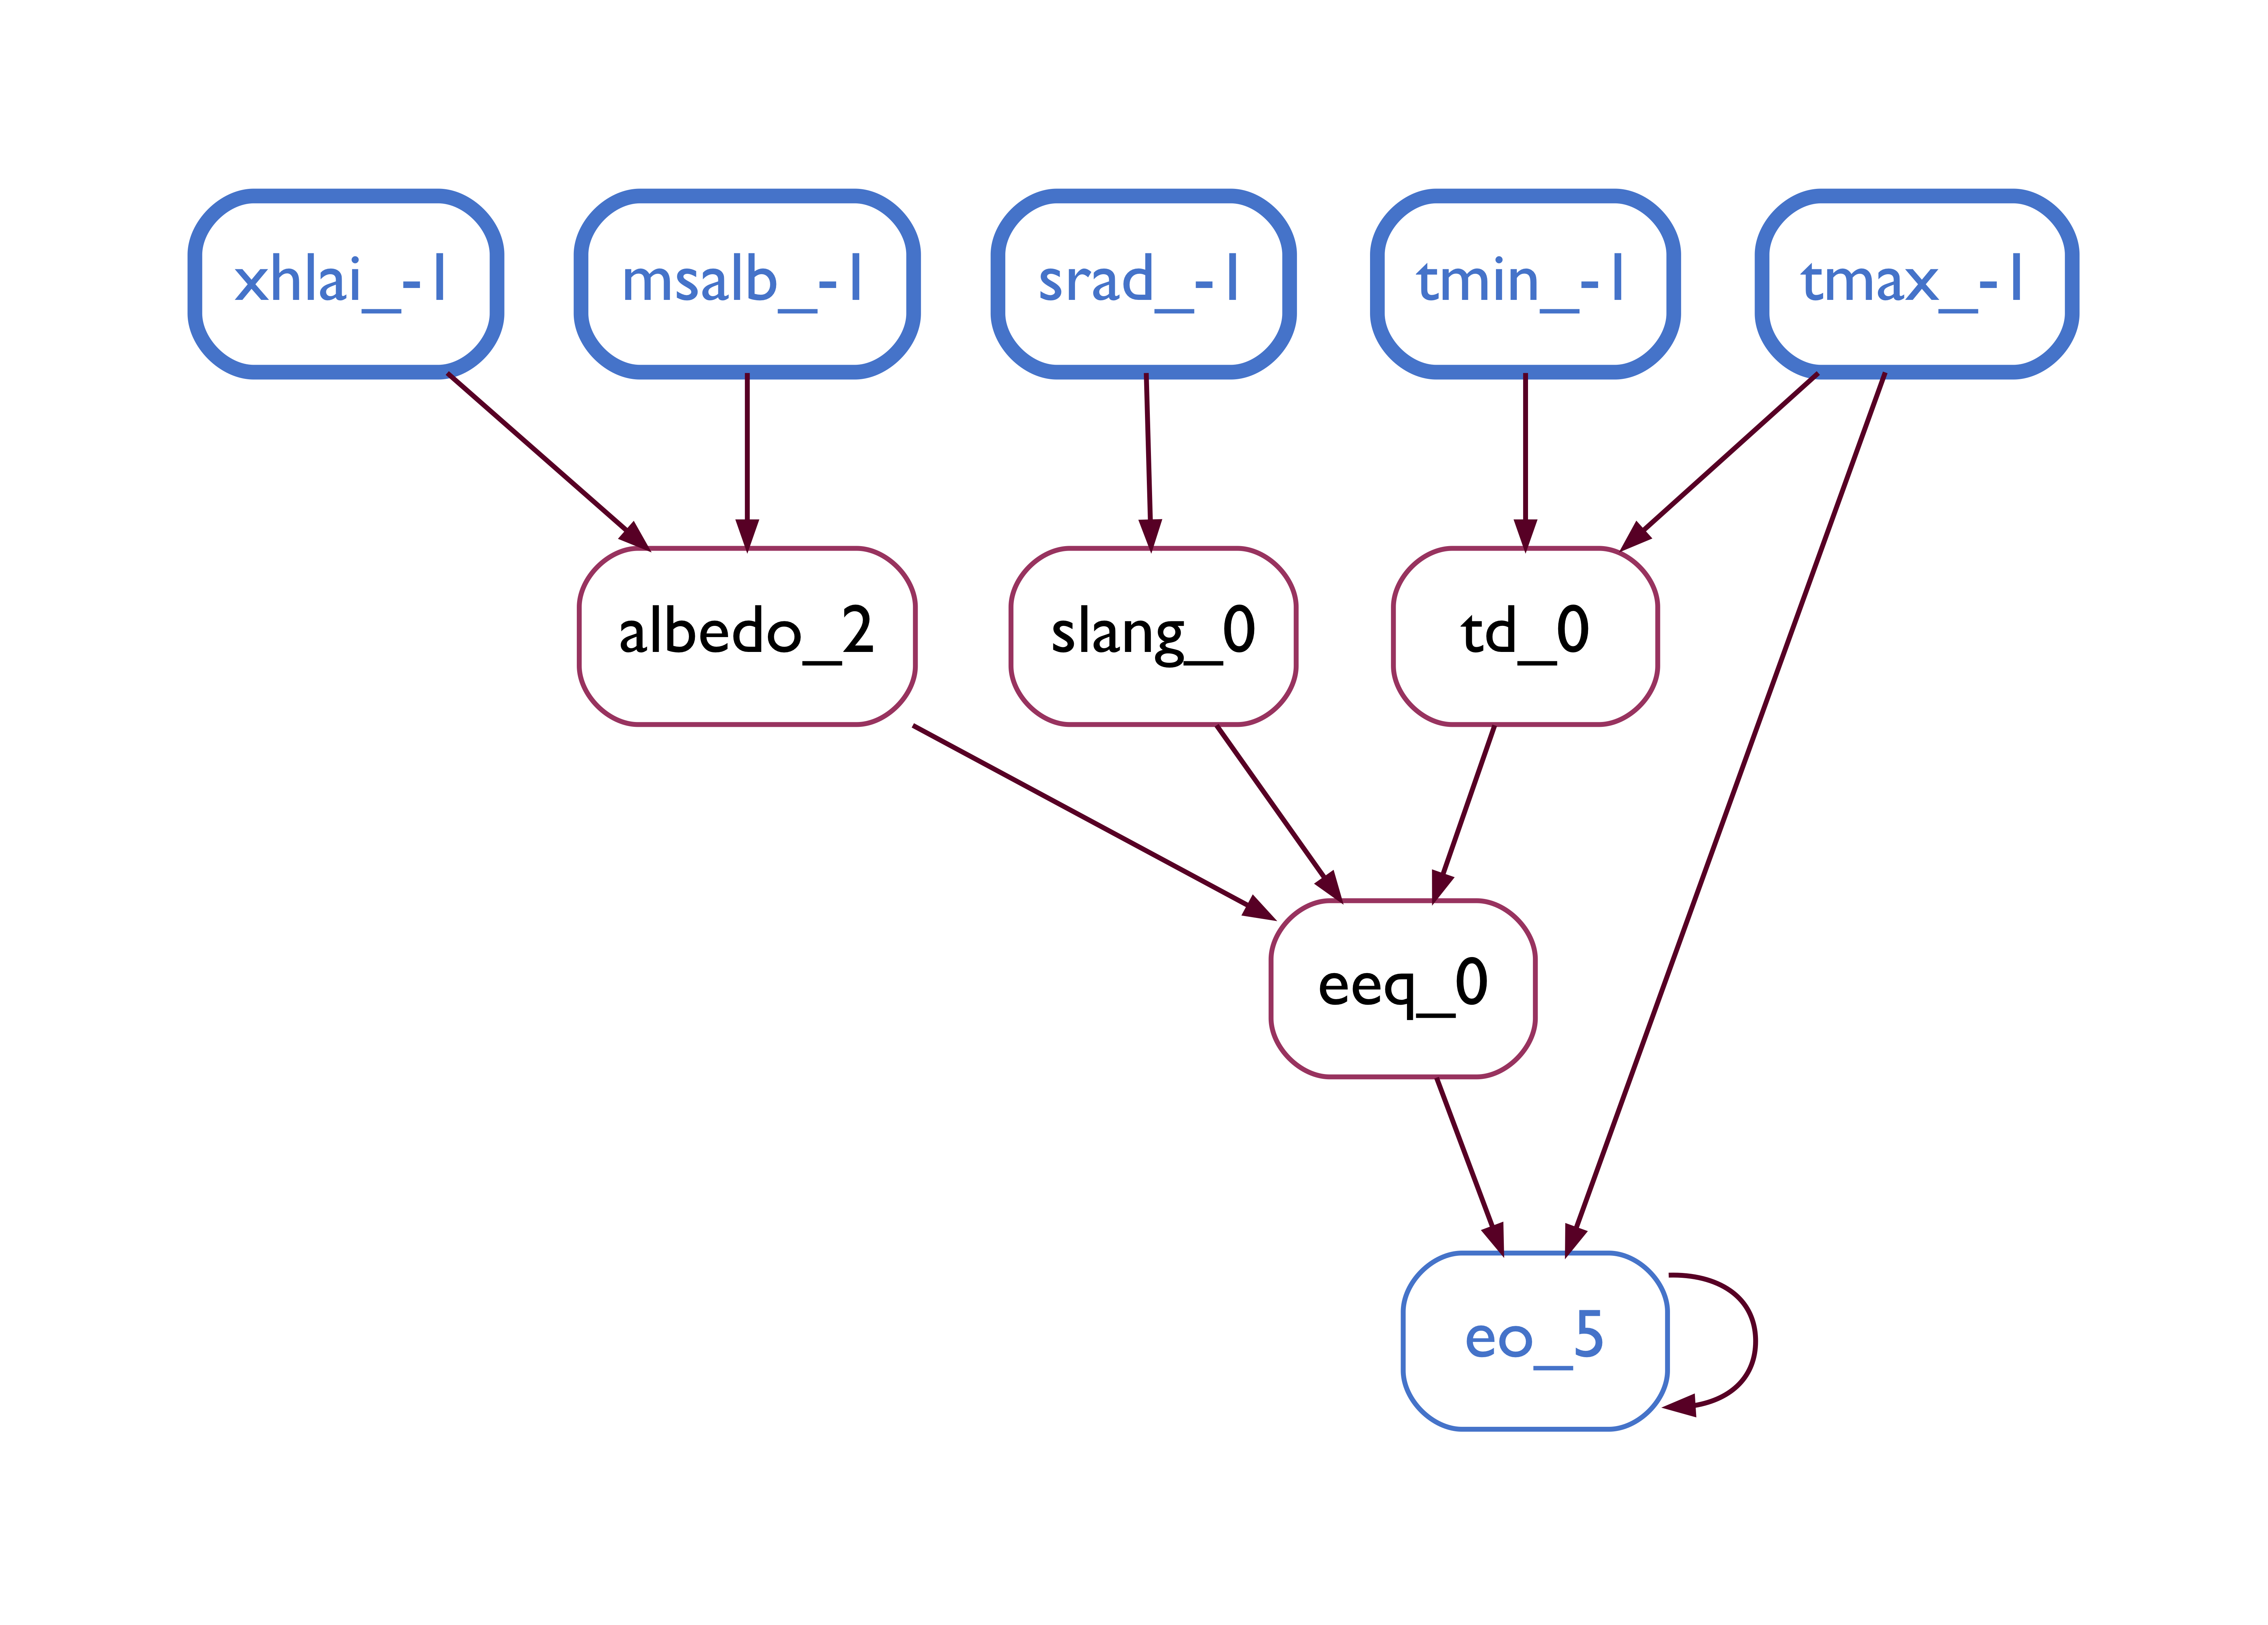
\includegraphics[clip,width=.8\columnwidth]{PETPT_FIB_CAG}%
%     \caption[PETPT FIB CAG]{A Forward Influence Blanket (FIB) for the PETPT model that depicts the overlap with the PETASCE model. Note that shared variables are shaded in blue and shared input variables are both shaded blue and bolded.}
% \end{figure}
%
% \begin{figure}[!htbp]
%     \label{petasce_fib}
%     \centering
%     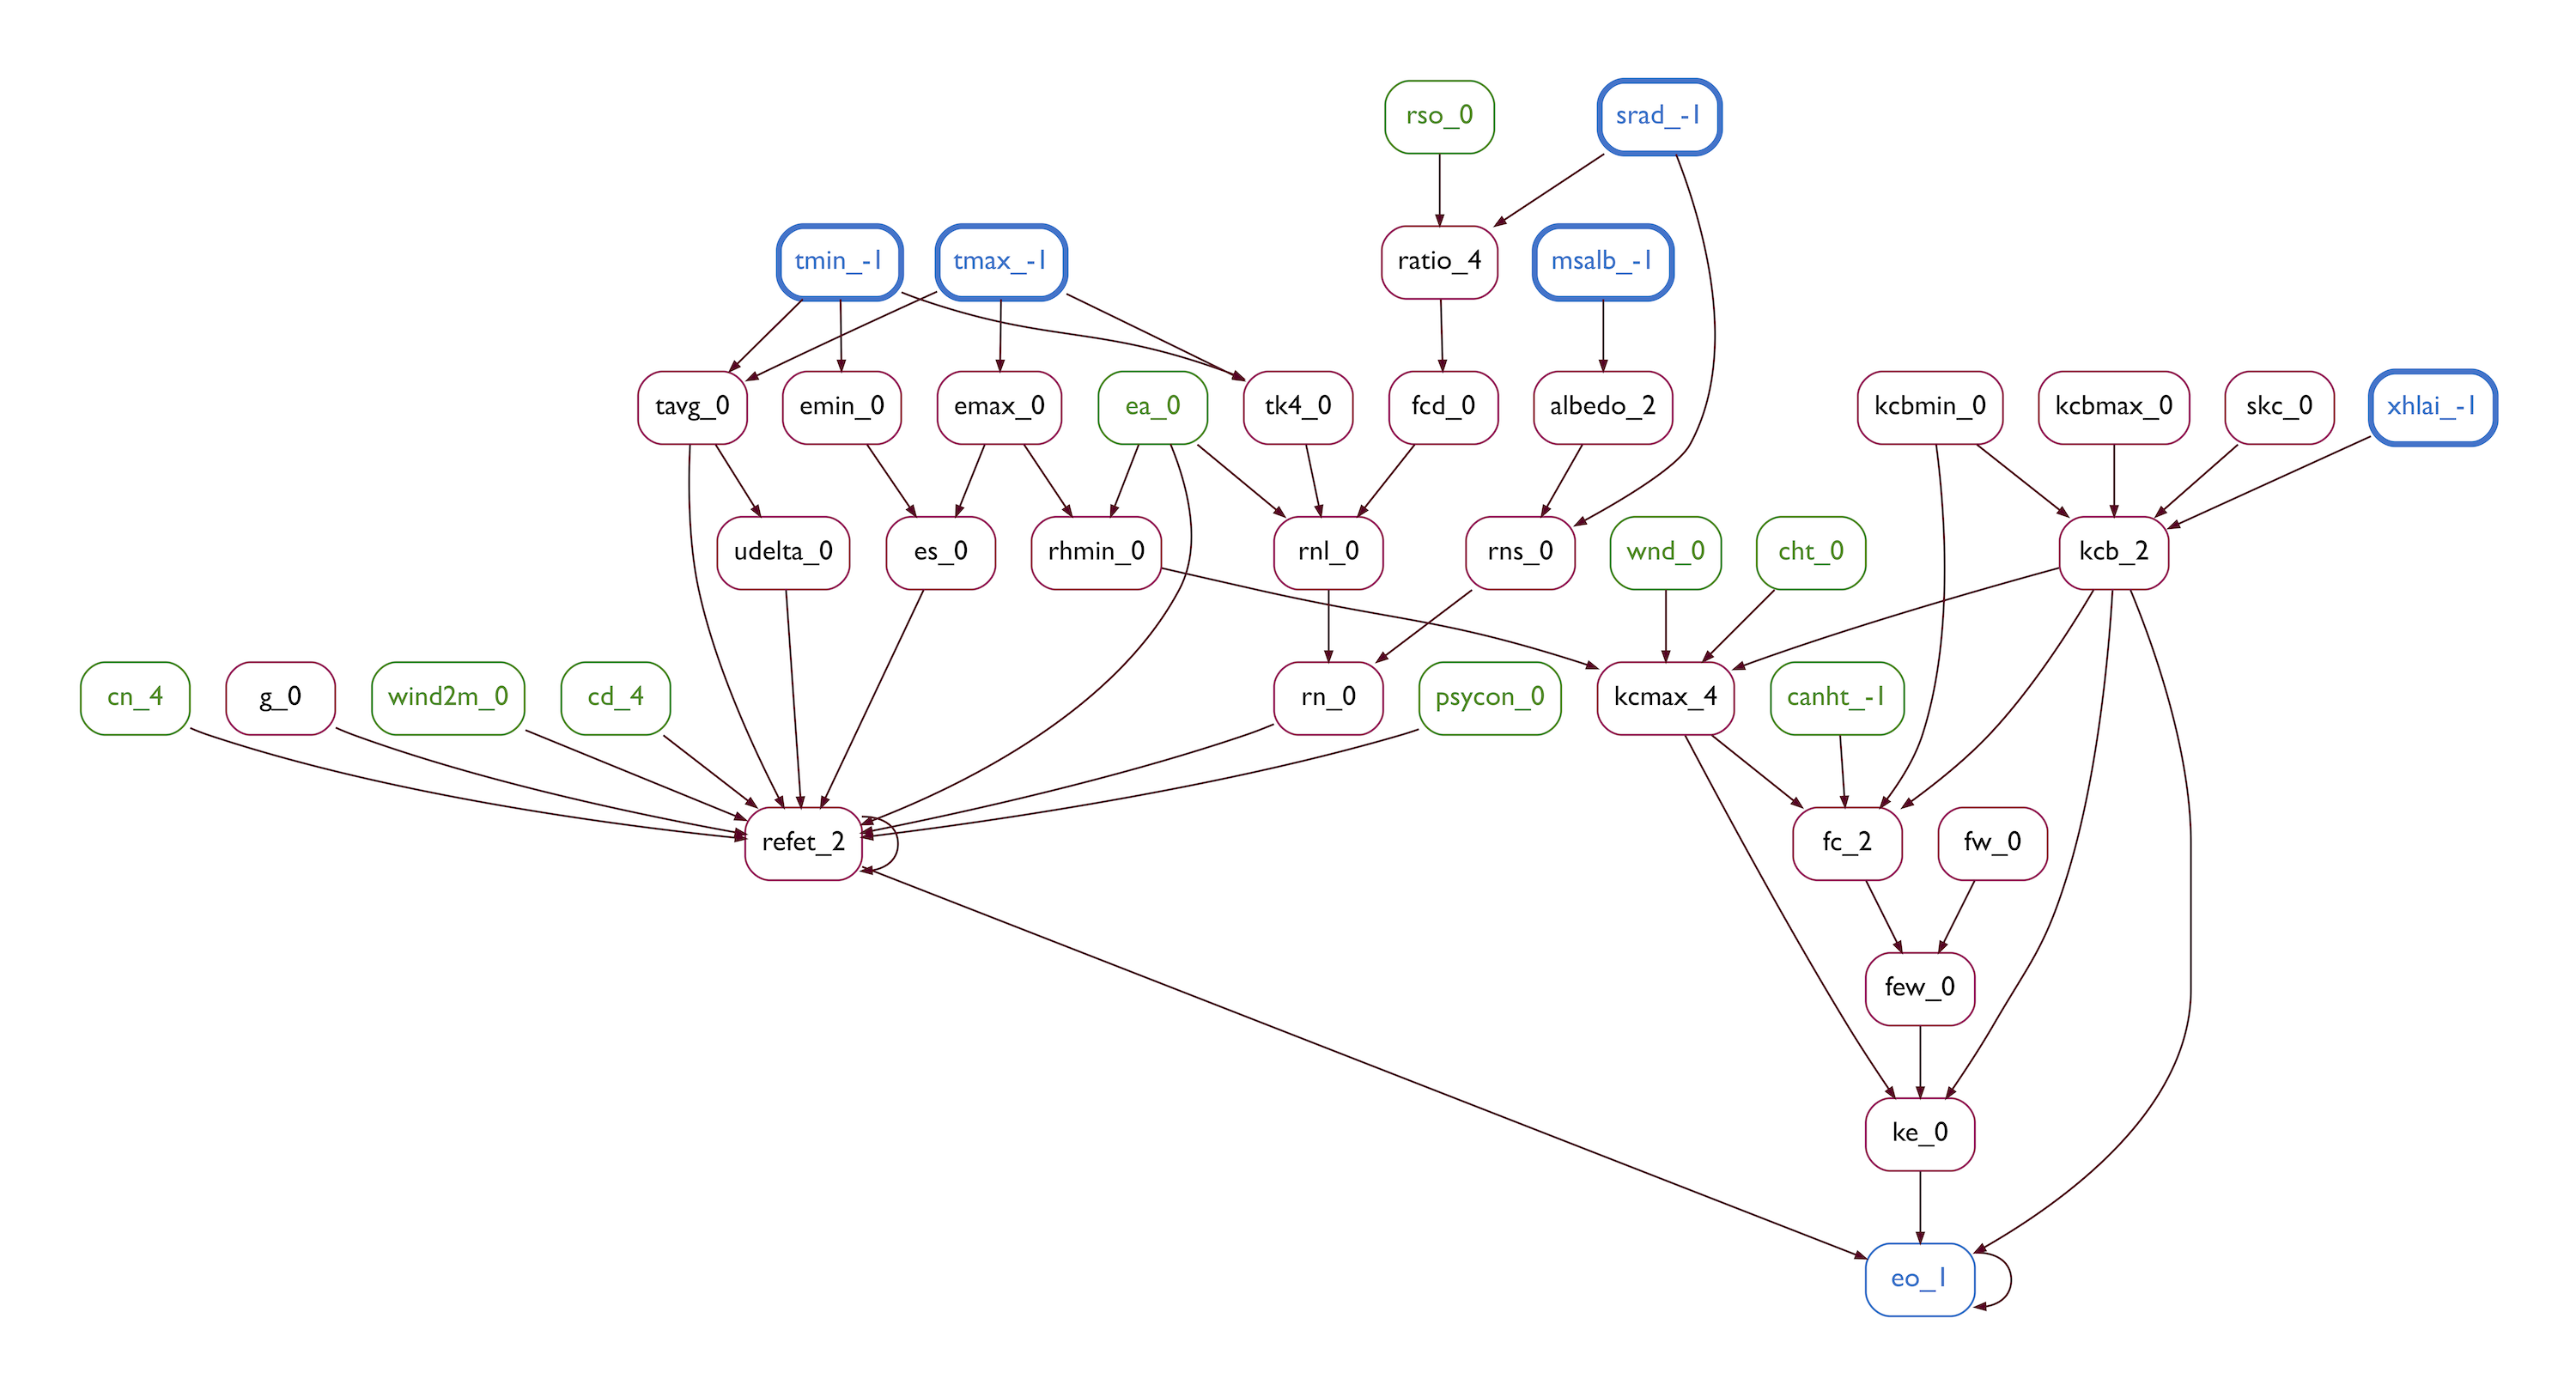
\includegraphics[clip,width=0.8\columnwidth]{PETASCE_FIB_CAG_smaller}%
%     \caption[PETASCE FIB CAG]{A Forward Influence Blanket (FIB) for the PETASCE model that depicts the overlap with the PETPT model. Note that while the PETPT model did not have any variable nodes in the cover set the PETASCE model has several variables in the cover set. These variables are shaded green.}
% \end{figure}
% \FloatBarrier

\subsection{Input Set Execution on a FIB\label{sec:fib_exec}}
In order to execute a FIB the user must provide values for the input variable nodes and values for the cover variable nodes. At execution time, both sets of variable nodes will be populated before beginning to compute the function nodes in the partial order of functions provided by the GrFN computation graph. This is the only difference between computing on a FIB computation graph and computing on a GrFN computation graph.

Execution of a FIB computation graph can be done either with singular preset values for all of the cover variables, or with ranges for each cover variable.
FIB CGs support Torch-aided vectorized computation similar to the GrFN CG structure, and no additional memory constraints are imposed on execution by the FIB class.
